\documentclass[a4paper,10pt]{article}
\pdfoutput=1 % if your are submitting a pdflatex (i.e. if you have
             % images in pdf, png or jpg format)
\usepackage{jcappub} % for details on the use of the package, please
                     % see the JCAP-author-manual          
\usepackage{enumitem}% http://ctan.org/pkg/enumitem
\usepackage[T1]{fontenc} % if needed
\usepackage{hyperref}

\graphicspath{ {images/} }



\renewcommand{\v}[1]{\mathbf{#1}}
\newcommand{\Mp}{M_{pl}}
\newcommand{\half}{\frac{1}{2}}
\newcommand{\bphi}{\bar{\phi}}
\newcommand{\ann}[1]{\hat{a}_{\v{#1}}}
\newcommand{\cre}[1]{\hat{a}^\dagger_{\v{#1}}}
\newcommand{\anns}[2]{\hat{a}_{\v{#1}#2}}
\newcommand{\cres}[2]{\hat{a}^\dagger_{\v{#1}#2}}
\newcommand{\vac}{|0 \rangle}
\newcommand{\fint}[1]{\int \frac{d^3 \v{#1}}{(2\pi)^3}}
\newcommand{\finttwo}[1]{\int \frac{d^2 \v{#1}}{(2\pi)^2}}
\newcommand{\unit}[1]{\hat{\v{#1}}}
\newcommand{\sr}{\text{\normalfont\dh}}
\renewcommand{\sl}{\bar{\text{\normalfont\dh}}}
\newcommand{\ltwo}{\left[\frac{(l+2)!}{(l-2)!}\right]}
\newcommand{\ltwof}{\left[\frac{(l-2)!}{(l+2)!}\right]}

\title{\boldmath The Search for CMB B-mode Polarization from Inflationary Gravitational Waves}


%% %simple case: 2 authors, same institution
%% \author{A. Uthor}
%% \author{and A. Nother Author}
%% \affiliation{Institution,\\Address, Country}

% more complex case: 4 authors, 3 institutions, 2 footnotes
\author{B. Chughtai}

% The "\note" macro will give a warning: "Ignoring empty anchor..."
% you can safely ignore it.

\affiliation{University of Cambridge, Cambridge, UK}


% e-mail addresses: one for each author, in the same order as the authors
\emailAdd{bc464@cam.ac.uk}




%\abstract{Abstract...}



\begin{document}
\maketitle
\flushbottom

%\section{Things to do/add}

%I note this essay currently sits on the longer side at around 13000 words so am not keen to add more. I could probably cut some sections and get it down to a more reasonable 10000 if necessary\\

%Things I could possibly add:
%explicit grav wave action expansion ~ 3 pages \\
%could flesh our discussion of features of power spectra a bit more - zhao and zeng \\
%TASI Notes: Current evidence for inflation ~ 1 page\\
%Derivation of LHS of boltzmann eqn for polarisation in presence of grav wave - including geodesic eqn ~ 2 pages\\
%some more about inflation and consequences for HEP

%\section{things done}
%instein eqn -> evolution of grav wave derivation ~ 1 page - found a better way
%why is lensing useful - hanson et al
%something about the born apporximation	 - hanson et al
%expand on correlation functions when doing series expansion in lensing chapter

\section{Introduction}


This essay focuses on early-universe cosmology. It explores an aspect of the age-old question ``Where do we come from?''. In particular, it asks ``What mechanism drove the first few moments of the universe, and how can we experimentally test that?''. Let us tackle each point in turn.\\

The present leading paradigm for these initial few moments of the Universe is that of inflation, a period of rapid accelerated expansion lasting only $\sim10^{-32}$s . Initially postulated by Guth in 1981 \cite{Guth} in order to solve some large conceptual holes in the previous hot Big Bang cosmology, it was soon realized it also provided a convenient method of generating the primordial density fluctuations necessary to seed the growth of large scale structure, setting the `initial conditions' for the universe. \\

Compared to the complexity of physics on the small scale, our cosmic landscape is rather simple - the cosmological principle states that on large scales we expect the universe as a whole to be homogeneous and isotropic. Were this true on all scales, life would not have formed, so it is fortunate this breaks down at some point - which is precisely what modern cosmology relies on. These tiny departures from homogeneity contain vasts amount of information about the universe's evolution. Over the past few decades an era of `precision cosmology' has been ushered in by ever more accurate measurements of the distribution of mass on cosmic scales through galaxy surveys, and through measurements of the temperature and polarization fluctuations of the cosmic microwave background (CMB). \\

We now return to inflation. The theory community has over the years produced hundreds of plausible models for inflation, with data now being required to validate or invalidate any particular one. The simplest, and indeed canonical models of inflation are those of so called single-field slow-roll (SFSR) - which generically make a number of predictions validated by increasingly precise measurements over the past two decades. Namely the present day spatial flatness of the universe to within 1\% and the approximate scale-free, adiabatic, and Gaussian nature of primordial density perturbations. There remains more we don't know about inflation than we do however. For instance, what is the physical mechanism behind it? How and why did it stop? Questions like these may only be answered by putting more stringent constraints on the theory space of permissible models. Finally there remains the question as to whether inflation even occurred in the first place - some believe more evidence is needed.\\

Turning to the subject of this essay, many inflationary models, including the simplest SFSR ones, predict the existence of a stochastic background of inflationary gravitational waves, generated through tensor-like quantum-fluctuations of the metric during inflation, which have yet to be detected. In this essay I hope to convince the reader that firstly, we know precisely how these should effect CMB observables, and therefore know how to detect them, and secondly that this detection really would provide strong evidence for inflation and give us insight into its physics. This method of detection will be through the `B-mode' polarisation of the CMB. Scalar (i.e. density) perturbations source temperature anisotropies in the CMB, as well as so called E-mode polarisation. Tensor perturbations on the other hand source temperature anisotropies, E mode polarisation and crucially, B mode polarisation too. The B mode diagnostic is therefore the most sensitive test we have for primordial tensor perturbations - uncontaminated by dominant primordial density perturbations. A detection of this `inflationary B mode signal' has been termed a `smoking gun' for inflation for precisely for this reason. So far we have made precise measurements of the temperature anisotropy and E mode signal, giving us strong constraints on primordial density perturbations, but have yet to detect these B modes from tensor perturbations. \\

Beyond this, a detection of a B mode signal gives us insight into the spectrum of primordial tensor perturbations. At present, a lack of detection has bounded the `tensor-to-scalar' ratio $r$ to less than 1 part in 10. We will see later $r$ is fundamentally linked to, among other things, the energy scale of inflation, allowing us to put strong constraints on the type of models allowed. A lack of detection of $r$ is not useless to us either - it will put more stringent upper bounds on $r$, invalidating certain classes of models which would predict large tensor amplitudes.\\

\subsection{Outline}

The structure of this essay is as follows. We begin by reviewing the basics of inflationary cosmology, and a derivation of its predictions in SFSR for the stochastic IGW background. We discuss the parameters commonly used to describe inflationary models. We then turn our attention to the CMB, reviewing the basics of CMB polarisation, and its mathematical description on the curved 2-sphere. We show from the Boltzmann equation formalism that tensor perturbations do indeed produce a non zero B mode signal, and derive their power spectrum, while showing on the other hand that scalar perturbations do not. We then show all is not as easy as it seems, and discuss some major complications in attempting to detect this signal: the issues of other possible primordial B modes, foregrounds, and gravitational lensing in some detail. Finally we return again to inflation, discussing some of the exciting implications a detection of an inflationary B mode signal would mean for the cosmology and high energy physics communities. 

\subsection{Conventions}

We use the mostly plus Lorentzian signature $(-,+,+,+)$ in which Greek letters ($\mu,\nu$,...) are used for spacetime indices, while latin latters ($i,j$,...) are used for spatial indices. The scale factor is denoted $a$, and conformal time by $\tau$, which is related to coordinate time by the relation $a(\tau)d\tau = dt$. Coordinate time derivatives are denoted $\dot{}$, and conformal time derivatives $'$, for example the hubble factor is $H=\frac{\dot{a}}{a}$ and the comoving Hubble factor $\mathcal{H}=\frac{a'}{a}$. We use natural units in which $\hbar=c=k_B=1$, and where the reduced Planck mass $\Mp = 1/\sqrt{8\pi G}$. Our Fourier convention is the inhomogenous one, where $f(\v{x}) = \fint{k} f_\v{k}e^{i\v{k}\cdot\v{x}}$ in 3D, and an analogous statement holds in 2D.


\newpage
\section{Inflationary Cosmology}

In this section we review the physics of inflation, and the relevant results which we later link to CMB observables.

\subsection{Inflation Basics}
A flat, homogeneous and isotropic universe is described by the Friedmann–Lemaître–Robertson–Walker (FLRW) metric, which in our sign convention takes form
\begin{equation}
\label{FLRW}
ds^2 = - dt^2 + a^2(t)d\v{x}^2 = a^2(\tau)(-d\tau^2+d\v{x}^2)
\end{equation}
Assuming General Relativity, it obeys the Einstein equation $G_{ab} = \frac{1}{\Mp^2} T_{ab}$, sourced by a perfect fluid with energy momentum tensor $T_{ab}$, which by homogeneity and isotropy must take form
\begin{equation}
\label{densityandpressure}
T^0_0 = - \rho(t) \quad T^0_i = 0 \quad T^i_j = P(t)\delta^i_j
\end{equation}
where we  identify $\rho(t)$ as the total energy density and $P(t)$ as the total pressure. We will consider one component, the inflaton field, to dominate.  Substituting \ref{FLRW} and \ref{densityandpressure} into the Einstein Equation we obtain the Friedmann equations
\begin{equation}
H^2 = \left(\frac{\dot{a}}{a}\right)^2 = \frac{1}{3\Mp^2}\rho
\tag{F1}
\label{F1}
\end{equation}
\begin{equation}
\dot{H} + H^2 = \frac{\ddot{a}}{a} = -\frac{1}{6\Mp^2}(\rho + 3P)
\tag{F2}
\label{F2}
\end{equation}
Inflation requires a shrinking hubble radius $\frac{d}{dt}\mathcal{H}^{-1}<0$, equivalent to \textit{accelerated expansion} $\ddot{a} >0$. We may define the first hubble slow roll parameter 
\begin{equation}
\label{epsilon}
\epsilon := -\frac{\dot{H}}{H^2} = -\frac{d\ln{H}}{d\ln{a}} = \frac{3}{2}\left(1+\frac{P}{\rho}\right)
\end{equation}
where the last inequality follows from the Friedmann Equations. We find $\ddot{a} >0$ is equivalent to $\epsilon<1$ or to the condition on the equation of state parameter $\omega=P/\rho < -1/3$.\\ 

In order to solve the horizon problem we require inflation to persist for a relatively long duration of time ($\sim$ 60 e-folds), so $\epsilon$ must remain small. We parametrise how quickly $\epsilon$ changes in the second hubble slow roll parameter 
\begin{equation}
\eta = -\frac{\dot{\epsilon}}{H\epsilon} = -\frac{d\ln{\epsilon}}{d\ln{a}}
\end{equation}
which we also require to be small during inflation.

\subsubsection{Single Scalar Field Dynamics}

The simplest class of inflation models are those consisting of a single scalar field, slowly rolling down its potential, minimally coupled to gravity. These postulate the existence of a single effective scalar degree of freedom - the ``inflation'' field $\phi(t,\v{x})$. The total action is given by
\begin{equation}
S = \frac{\Mp^2}{2} \int d^4x \sqrt{-g}[R+2P(X,\phi)] 
\label{inflationaction}
\end{equation}
for $X=-\half g^{\mu\nu}\partial_\mu\phi\partial_\nu\phi$. Slow roll inflation corresponds to a canonical kinetic term 
\begin{equation}
P(X,\phi) = X - V(\phi)
\end{equation}
where all inflationary dynamics are specified by the potential $V(\phi)$. Inserting the energy momentum tensor for the matter Lagrangian into \ref{densityandpressure} and the Friedmann equations \ref{F1}, \ref{F2} we obtain the equations of motion for the classical background $\phi(t)$
\begin{equation}\begin{split}
H^2 &= \frac{1}{3\Mp^2}\left(\half\dot{\phi}^2+V(\phi)\right)\\
\frac{\ddot{a}}{a} &= -\frac{1}{3\Mp^2}\left(\dot{\phi}^2-V(\phi)\right)\\
\end{split}\end{equation}
giving the Klein Gordon equation
\begin{equation}
\tag{KG}
\label{KG}
\ddot{\phi}+3H\dot{\phi}=-V_{,\phi}
\end{equation}
From these we see the spacetime axperiences accelerated expansion iff the potential energy dominates the kinetic: $V > \dot{\phi}^2$ and is sustained if $|\ddot{\phi}| \ll |V_{,\phi}|$. We also find that by \ref{epsilon} that 
\begin{equation}
\epsilon = \frac{1}{\Mp^2}\frac{\half\dot{\phi}^2}{H^2} < 1
\end{equation}

\subsubsection{Slow Roll}

The slow roll approximation postulates the kinetic energy and acceleration of the background field is much smaller than its potential energy, encapsulated in terms of our slow roll parameters as $(\epsilon, \eta \ll 1)$. In this approximation we get by \ref{F1} and \ref{KG} 
\begin{equation}\begin{split}
H^2 &\approx \frac{V}{3\Mp^2} \\
3H\dot{\phi} &\approx -V_{,\phi}
\end{split}\end{equation}
from which we see 
\begin{equation}
\epsilon \approx \half\Mp^2 (\frac{V'}{V})^2 := \epsilon_V
\end{equation}
where we have defined the first \textit{potential} slow roll parameter. We can analogously define a second potential slow roll parameter via
\begin{equation}
\eta_V = \Mp^2 \frac{V''}{V} \approx 2\epsilon - \half\eta
\end{equation}
which must therefore also be small. With these constraints satisfied, inflation occurs and inflates the universe in a quasi-deSitter fashion
\begin{equation}
a(t) \approx a(0)e^{Ht} \qquad H\approx\text{constant}
\end{equation} 
Since $\phi$ acts as a clock during inflation, we may express the number of e-folds of inflation from a time $t$ until the end of inflation as an integral over field excursion instead of time
\begin{equation}
N(t) := \ln{\frac{a(t_{end})}{a(t)}} = \int_a^{a(t)} d(\ln{a}) = \int_t^{t_{end}} Hdt = \int_{\phi(t)}^{\phi_{end}} \frac{d\phi}{\sqrt{2\epsilon}\Mp}
\label{efolds}
\end{equation}
using $Hdt=\frac{H}{\dot{\phi}}d\phi=\frac{d\phi}{\sqrt{2\epsilon}\Mp}$


\subsection{Cosmological Perturbation Theory}
So far we have only considered the homogeneous and isotropic background for the inflaton. In general it can also vary in space, as can the metric, which also experiences perturbations following \cite{CMBPol}.
\begin{equation}
\phi(t,\v{x}) = \bphi(t) +\delta\phi(t,\v{x}) \qquad g_{\mu\nu}(t,\v{x}) = \bar{g}_{\mu\nu}(t,\v{x}) +\delta g_{\mu\nu}(t,\v{x})
\end{equation}
where the metric can be written
\begin{equation}
\begin{split}
ds^2 &= g_{\mu\nu}dx^\mu dx^\nu\\
&= -(1+2\Phi)dt^2 + 2aB_idx^idt+a^2[(1-2\Psi)\delta_{ij}+E_{ij}]dx^idx^j
\end{split}
\label{metricperturb}
\end{equation}

We now perform the Scalar-Vector-Tensor decomposition, writing
\begin{align}
B_i &= \partial_i B - B_i, \quad \partial^iB_i=0\\
E_{ij} &= 2\partial_{ij}E + 2\partial_{(i}E_{j)} + h_{ij}, \quad \partial^iE_i=0, \quad h^i_i = \partial^ih_{ij}=0
\end{align}

Crucially, at linear order, scalars, vectors and tensors evolve independently, and so can be treated separately. It is also useful to work in Fourier space, since as always distinct Fourier modes decouple at linear order. Importantly the perturbations $\delta\phi$ and $\delta g_{\mu\nu}$ are gauge dependent, and mix the scalars, vectors and tensors separately under coordinate transformations. We therefore must either work in a fixed gauge or use gauge invariant quantities.\\

\textbf{Scalars} - An important gauge invariant quantity is the comoving curvature perturbation
\begin{equation}
-\zeta = \Psi + \frac{H}{\dot\rho}\delta{\rho} 
\label{zeta}
\end{equation}
for $\rho$ the total energy density of the universe. In a gauge where $\delta{\rho}_\phi = 0$ all scalar degrees of freedom during inflation can be expressed by a single metric perturbation 
\begin{equation}
g_{ij} = a^2(t)[1+2\zeta]\delta_{ij}
\end{equation}
where the 3 dimensional Ricci scalar of constant density hypersurfaces is given by $\mathcal{R}^{(3)} = -4\nabla^2\zeta / a^2$. It turns out $\zeta$ is conserved outside the horizon \cite{baumann}, important since during inflation modes eventully exit the horizon, re-entering at a time after inflation ends and the horizon has grown again, and so can be thought of as `freezing out'. In the spatially flat gauge, $\zeta$ is simply the dimensionless density perturbation, and one can construct transfer functions relating the late time evolved values of cosmological fields to this initial frozen value of $\zeta$. \\

Thus $\zeta$ is the relevant quantity to describe primordial scalar perturbations. It's dimensionless power spectrum is
\begin{equation}
\langle \zeta(\v{k})\zeta(\v{k'}) \rangle=(2\pi)^3\delta(\v{k}+\v{k'})\frac{2\pi^2}{k^3}\Delta^2_s(k)
\end{equation}
with scale dependence described by the scalar spectral index
\begin{equation}
n_s-1 = \frac{d\ln{\Delta^2_s}}{d\ln{k}}
\end{equation}
giving the approximate form 
\begin{equation}
\Delta^2_s(k) \approx A_s(k_*)(\frac{k}{k_*})^{n_s-1} 
\end{equation}
where $k_*$ is some pivot scale. \\


\textbf{Vectors} - It can be shown vectors decay rapidly as the universe expands, and may be neglected as they are not expected to contribute significantly to the relevant CMB observables if generated during inflation. There are exceptions to this, see section \ref{vectorissues}.\\

\textbf{Tensors} - Since there is only one tensor $h_{ij}$, it must be gauge invariant. This term is in essence responsible for the content of the rest of the essay - it describes primordial gravitational waves. The relevant quantity to consider is again the power spectrum

\begin{equation}
\langle h_{ij}(\v{k})h_{ij}(\v{k'}) \rangle=(2\pi)^3\delta(\v{k}+\v{k'})\frac{2\pi^2}{k^3}\Delta^2_t(k)
\label{tensorpowerspec}
\end{equation}

It's scale dependence is defined analogously as 

\begin{equation}
n_t = \frac{d\ln{\Delta^2_t}}{d\ln{k}}
\end{equation}

giving the approximate form 

\begin{equation}
\Delta^2_t(k) \approx A_t(k_*)(\frac{k}{k_*})^{n_t}
\end{equation}

We can now define the important parameter $r$, the tensor to scalar ratio.

\begin{equation}
r(k_*)=\frac{A_t(k_*)}{A_s(k_*)} 
\end{equation}

\subsection{SFSR Power Spectra}

The scalar and tensor power spectra are model dependent. We compute them in the SFSR regime in appendix \ref{SFSRderivation}, with key results being

\begin{equation}
\Delta^2_{s}(k) = \frac{1}{2\epsilon\Mp^2}\left(\frac{H}{2\pi}\right)^2\rvert_{k=aH} \qquad
\Delta^2_t(k)= \frac{2}{\pi^2}\left(\frac{H}{\Mp}\right)^2\rvert_{k=aH}
\end{equation}

These power spectra provide the initial conditions of the universe. Given a good understanding of the physics of proceeding cosmological evolution we have several direct probes of these power spectra. Later sections of this essay will go into more detail about signatures of the tensor power spectrum in particular.\\

Here we investigate some of their properties. Recall H is approximately constant during inflation, but not perfectly so, since $H^2 \sim V(\phi)$, and $\phi$ is slowly rolling down its potential. Similarly $\epsilon$ also varies slightly, and so we expect slight scale invariance from $n_s-1\approx0$, $n_t\approx0$. We can compute the spectral indices in terms of the slow roll parameters. 
\begin{equation}\begin{split}
n_s-1 &= \frac{d\ln{\Delta^2_s}}{d\ln{k}} = \frac{d}{d\ln{k}}(2\ln{H}-\ln{\epsilon}) \approx \frac{1}{H}\frac{d}{dt}(2\ln{H}-\ln{\epsilon}) = \frac{2\dot{H}}{H^2}-\frac{\dot{\epsilon}}{H\epsilon}\\
& = -2\epsilon-\eta = -6\epsilon_V+2\eta_V\\
n_t &= \frac{d\ln{\Delta^2_t}}{d\ln{k}} = \frac{d}{d\ln{k}}2\ln{H}\\
&=-2\epsilon=-2\epsilon_V
\end{split}\end{equation}

where we have used that $d\ln{k} = d\ln{aH} \approx d\ln{a} = Hdt$ since we evaluate the power spectra at horizon exit, and H is slowly varying (so $d\ln{H}$ provides a next to leading order correction). During inflation $\epsilon>0$ since energy density is monotonically decreasing, and so $n_t<0$ and tensor perturbations are said to have a red spectrum. $n_s$ on the other hand can have either a red ($n_s<1$) or blue ($n_s>1$) spectrum. The scalar to tensor ratio can be computed as

\begin{equation}
r=\frac{A_t}{A_s} \approx 16\epsilon
\end{equation}

leading to the consistency condition $r=-8n_t$, which serves as a test, at least in principle, of SFSR.


\subsection{Current Observational Constraints}


A number of inflationary parameters have been measured through CMB experiments. From Planck 2018 temperatuere, polarisation and lensing data at 68\% confidence and for the purposes of this essay, the relevant parameters include \cite{Planck}
 
\begin{itemize}
\item A red tilted scalar spectral index $n_s =0.9649 \pm 0.0042$, with no evidence for scale dependence of $n_s$. The perfectly scale invariant $n_s=1$ spectrum is ruled out by more than $8\sigma$, providing strong evidence for inflation
\item A scalar amplitude  $10^9 A_s \approx 2.100 \pm 0.030$
\end{itemize}

We have not yet made a detection of any primordial tensor perturbations, and only have an upper limit on the tensor to scalar ratio $r_{0.002}<0.10$ from Planck data alone, or $r_{0.002}<0.056$ by also making use of the BICEP2/Keck Array BK15 data \cite{planck-inflation}. We obviously have no bounds on $n_t$.\\

In order to get a better understanding of the physics of inflation, we would really like to get a better constraint on $r$ initially, and $n_t$ in future. We explore the physics implication of these parameters later in \ref{probe}, though we first must explain how on earth we are going to measure them.

\newpage

\section{The B Mode Diagnostic}

We now turn to how we go about measuring r. Our best method for doing so is through the CMB. The CMB exhibits temperature (T) anisotropies, but also turns out to be partially polarised. While Thomson scattering of isotropic radiation would produce no polarisation, the CMB possesses a quadrupolar ($Y_{2m}$) variation in temperature, which gives rise to linear polarisation upon scattering. When Thomson scattering is rapid, the randomization of photon directions destroys any quadrupole anisotropy and polarization. The problem of understanding the polarization pattern of the CMB thus reduces to understanding the quadrupolar temperature fluctuations when the rate has suffiecently slowed, i.e. at last scattering \cite{hu}. Polarisation turns out to be a more direct probe of the last scattering epoch than temperature, since it is unaffected by later universe `integrated' effects. In this section we first introduce the formalism in which we may define polarisation fields on the full sky, and then compute using the line of sight method the power spectrum for B modes arising from primordial tensor perturbations, which we find to be non zero. In contrast we show scalar perturbations don't produce any B modes, instead only contributing to the T and E power spectra. Thus, a measurement of a non zero B mode signal gives us a clean direct probe of the primordial tensor power spectrum, and $r$. 

\subsection{CMB Observables}

%TODO somethings wrong here
A CMB Photon detector measures the electric field $\v{E}$ perpendicular to the direction of observation $\hat{\v{n}}$, from which we can definite a rank two intensity correlation tensor following for example \cite{baldauf,lewis}.

\begin{equation}
I_{ij} = \langle E_aE_b^* \rangle
\end{equation}

where $\langle\rangle$ denotes a time average over several periods, where the amplitude changes insignificantly. Rank two tensors can be decomposed into three irreducible components: a trace part, a symmetric trace free part, and an antisymmetric part.  Fixing an orthonormal basis $\{\unit{e_1},\unit{e_2}\}$ orthogonal to the line of sight $\unit{n}$ we encode the four degrees of freedom as 

%\begin{equation}
%I_{ij} = T\delta_{ij}+2P_{ij}
%=\half\begin{pmatrix}
%T+Q & U\\ 
%U & T-Q
%\end{pmatrix}
%\end{equation}

\begin{equation}
I_{ij} =
\half\begin{pmatrix}
I+Q & U+iV\\ 
U-iV & I-Q
\end{pmatrix}
\end{equation}
The antisymmetric part encodes a phase lag between $E_1$ and $E_2$, i.e. circular polarization $V$. Thomson scattering induces no such polarisation, since the relevant boltzmann equation has no source term, and so we may neglect this \cite{kowosky}. The polarisation matrix is therefore 
\begin{equation}
P_{ij} =\half \begin{pmatrix}
Q & U\\ 
U & -Q
\end{pmatrix}
\end{equation}
Q and U are standard Stokes' parameters, which are functions of frequency and direction in general. In linear theory, their frequency dependence follows that of temperature anisotropies. We therefore normalize Q and U with respect to temperature rather than intensity, by dividing by the derivative of the CMB blackbody brightness with respect to log temperature to get frequency independent fractional thermodynamic equivalent temperatures, denoted $Q(\unit{n})$ and $U(\unit{n})$ \cite{notes}. \\

The Q parameter can be though of as the difference in power measured between an observer aligned with $\unit{e}_1$ and $\unit{e}_2$ while U can be thought of as the difference between $\unit{e}_1\pm\unit{e}_2$. Note $P_{ij}$ has eigenvalues $\pm (Q^2 + U^2)^\half$, with magnitude the polarisation amplitude, with corresponding eigenvectors making an angle of $\half\arctan(\frac{U}{Q})$ with $\unit{e}_1$. Diagrammatically, we may therefore depict polarisation as headless vectors of length $(Q^2 + U^2)^\half$, making an angle of $\half\arctan(\frac{U}{Q})$ to $\unit{e}_1$, so that the direction indicates the axis of measurement maximising measured signal.\\

Since $\delta_{ij}$ is the unique symmetric tensor invariant under rotations we see that $I$ is invariant under rotations, but $Q$ and $U$ are not. In particular if we perform a right handed rotation around $\unit{n}$ by an angle $\psi$ we get the following transformations
\begin{equation}
\begin{pmatrix}
\unit{e}_1'\\
\unit{e}_2' 
\end{pmatrix}
=
\begin{pmatrix}
\cos{\psi} & \sin{\psi}\\ 
-\sin{\psi} & \cos{\psi}
\end{pmatrix}
\begin{pmatrix}
\unit{e}_1\\
\unit{e}_2
\end{pmatrix}
\end{equation}


\begin{equation}
\begin{pmatrix}
Q'\\
U' 
\end{pmatrix}
=
\begin{pmatrix}
\cos{2\psi} & \sin{2\psi}\\ 
-\sin{2\psi} & \cos{2\psi}
\end{pmatrix}
\begin{pmatrix}
Q\\
U
\end{pmatrix}
\label{QUtranform}
\end{equation}

The fact that Q and U are basis dependent is a nuisance:  they aren't physical, and cannot be compared meaningfully at different points on the sphere. The polarisation tensors live in different vector spaces: entirely analogous with the same concept in differential geometry. \\

It is convenient to instead work with complex quantities $Q\pm iU$, equivalent to working in the complex basis $\unit{e}_\pm = \frac{1}{\sqrt{2}}(\unit{e}_1 \pm i\unit{e}_2)$ in which the polarisation tensor is diagonal. Using \ref{QUtranform}, it is easy to see under rotation this quantity transforms more simply as
\begin{equation}
Q'\pm iU' = e^{\mp 2i\psi}(Q\pm iU)
\end{equation}

Now a definition: A function $f(\theta, \phi)$ defined on a sphere is said to have \textit{spin $s$} if under a right handed rotation by angle $\psi$ of orthogonal vectors $(\unit{e}_1, \unit{e}_2)$ tangential to the sphere , it transforms as $f'(\theta, \phi) = e^{-is\psi}f(\theta, \phi)$. A spin 0 quantity is therefore a scalar under rotations. Note these rotations are not of the sphere, but instead of the tangent space orthogonal to $\unit{n}$.\\

Thus $Q+iU$ is a spin $2$ quantity, $Q-iU$ a spin $-2$ quantity, and $T$ a spin $0$ quantity. From here on out we use the natural choice of tangential basis at a point along line of sight $\unit{n} \equiv (\theta, \phi)$ on the sphere: $(\unit{e}_1, \unit{e}_2) = (\unit{e}_\theta, \unit{e}_\phi)$. Apart from the neater transformation law, the main reason we construct these quantities of definite spin is that analogously to the expansion of scalar quantities such as the temperature anisotropy in terms of spherical harmonics
\begin{equation}
T(\unit{n}) = \sum_{lm} T_{lm}Y_{lm}(\unit{n})
\end{equation}

there also exist `spin weighted spherical harmonics' $_sY_{lm}$ forming a complete orthonormal basis for spin s weighted functions \cite{all-sky}. Properties of these functions, and their relation to standard spherical harmonics are listed in Appendix \ref{swf}. In terms of these we may expand
\begin{equation}
(Q\pm iU)(\unit{n}) = \sum_{lm} a_{\pm2,lm} {}_{\pm2}Y_{lm}(\unit{n})
\label{QUexp}
\end{equation}

By reality conditions on $T, Q$ and $U$, we have
\begin{equation}
T_{lm}^* = T_{l,-m} \qquad a_{-2lm}^*=a_{2lm}
\end{equation}

We now solve our problem of coordinate dependence of Q and U by introducing spin raising ($\sr$) and lowering  ($\sl$) operators, which raise or lower the spin weight of a function by 1. Their properties, and explicit forms may be found in Appendix \ref{swf}. We construct two rotationally invariant scalar quantities out of $Q\pm iU$ by acting twice on \ref{QUexp} with our raising and lowering operators
\begin{equation}\begin{split}
\sr^2(Q-iU)(\unit{n}) &= \sum_{lm} \ltwo^{1/2} a_{2,lm} {}Y_{lm}(\unit{n})\\
\sl^2(Q+iU)(\unit{n}) &= \sum_{lm} \ltwo^{1/2} a_{-2,lm} {}Y_{lm}(\unit{n})
\end{split}\end{equation}

where now we can express $a_{\pm2,lm}$ using orthogonality of (spin weighted) spherical harmonics
\begin{equation}\begin{split}
a_{2,lm} &= \int d\Omega {}_2Y_{lm}^*(\unit{n})(Q+iU)(\unit{n})\\
&= \ltwo^{-1/2}\int d\Omega Y_{lm}^*(\unit{n})\sl^2(Q+iU)(\unit{n})\\
a_{-2,lm} &= \int d\Omega {}_2Y_{lm}^*(\unit{n})(Q-iU)(\unit{n})\\
&= \ltwo^{-1/2}\int d\Omega Y_{lm}^*(\unit{n})\sr^2(Q-iU)(\unit{n})
\end{split}\end{equation}

We construct two linear combinations of these modes, the physical $E$ and $B$ modes. The choice of sign here follows that of \cite{all-sky}, but note some authors make a different sign choice. For the purposes of calculating power spectra the choice does not matter.

\begin{equation}\begin{split} 
E_{lm} &= -(a_{2,lm} + a_{-2,lm})/2\\
B_{lm} &= i(a_{2,lm} - a_{-2,lm})/2
\end{split}\end{equation}
Using these we can rewrite \ref{QUexp} as 
\begin{equation}
(Q\pm iU)(\unit{n}) = -\sum_{lm} (E_{lm} \pm i B_{lm}) {}_{\pm2}Y_{lm}(\unit{n})
\label{QUEB}
\end{equation}

For real space calculations we introduce related quantities, which are manifestly rotationally invariant
\begin{equation}\begin{split}
\tilde{E}(\unit{n}) &:= -\half[\sl^2(Q+iU) + \sr^2(Q-iU)]\\
&= \sum_{lm} \tilde{E}_{lm}Y_{lm}(\unit{n})\\
&= \sum_{lm} \ltwo^{1/2}E_{lm}Y_{lm}(\unit{n})\\
\tilde{B}(\unit{n}) &:= \frac{i}{2}[\sl^2(Q+iU) - \sr^2(Q-iU)]\\
&= \sum_{lm} \tilde{B}_{lm}Y_{lm}(\unit{n})\\
&= \sum_{lm} \ltwo^{1/2}B_{lm}Y_{lm}(\unit{n})
\label{EBmodes}
\end{split}\end{equation}

$E$ and $B$ carry the same two degrees of freedom in polarisation that $Q$ and $U$ did, but are a lot nicer: they are defined in terms of scalars, and so are rotationally invariant, and therefore carry physical meaning.

\subsubsection{Parity}

We show here $E$ and $B$ have opposite parity. Consider a space inversion reversing the sign of the x coordinate. In spherical coordinates this leaves $r, \theta$ invariant, but varies $\phi \rightarrow -\phi$.  Let $\unit{n}\equiv(\theta, \phi)$ and $\unit{n}'\equiv(\theta', \phi')$ refer to the same physical direction in the two frames. From the definition of the Stokes parameters $Q=\langle |E_x|^2 \rangle - \langle |E_y|^2 \rangle$ and $U = \langle E_xE_y^* \rangle + \langle E_yE_x^* \rangle$ we see $Q'(\unit{n}') = Q'(\unit{n})$ but $U'(\unit{n}') = -U(\unit{n})$. Thus $(Q\pm iU)'(\unit{n}') = (Q\mp iU)(\unit{n})$. Now by \ref{EBmodes} we should act with spin raising and lowering operators twice. Acting once, using \ref{explicitspinraiselower}
\begin{equation}\begin{split}
\sl(Q+iU)'(\unit{n}') &= -\sin^{-2}{\theta'}[\partial_{\theta'}-i\csc{\theta'}\partial_{\phi'}]\sin^{2}{\theta'}(Q+iU)'(\unit{n}')\\
&= -\sin^{-2}{\theta}[\partial_{\theta}+i\csc{\theta}\partial_{\phi}]\sin^{2}{\theta}(Q-iU)'(\unit{n})\\
&= \sr (Q-iU)(\unit{n})
\end{split}\end{equation}
applying the operator once more gives
\begin{equation}
\sl^2(Q+iU)'(\unit{n}') = \sr^2 (Q-iU)(\unit{n})
\end{equation}
and similarly
\begin{equation}
\sr^2(Q-iU)'(\unit{n}') = \sl^2 (Q+iU)(\unit{n})
\end{equation}
so we see from \ref{EBmodes} that under parity $\tilde{E}'(\unit{n}')=\tilde{E}(\unit{n})$ but $\tilde{B}'(\unit{n}')=-\tilde{B}(\unit{n})$. Using the parity property of spherical harmonics $Y_{lm}\rightarrow(-1)^lY_{lm}$, we find that under a parity transformation multipoles transform as
\begin{equation}
E_{lm} \rightarrow (-1)^lE_{lm} \qquad B_{lm} \rightarrow (-1)^{l+1}B_{lm} \qquad T_{lm} \rightarrow (-1)^lT_{lm}
\end{equation} 

This property is the important distinguishing feature of E and B modes, and explains the nomenclature. It is in analogy with the electric and magnetic field, which transform as $E\rightarrow E$ and $B\rightarrow -B$ under parity too. We can use this property to distinguish E and B modes diagrammatically.

\begin{figure}[h]
  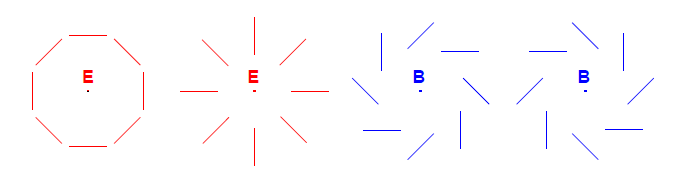
\includegraphics[width=\linewidth]{EBpicture.png}
  \caption{Typical E or B mode polarisation patterns. The electric and magnetic modes are distinguished by their behaviour under reflection.}
\end{figure}

\subsubsection{Statistics}

In this section we define the angular power spectra of interest. Since primordial perturbations from inflation are expected to be Gaussian, and since we expect linear theory to be a very good approximation in the early universe pre recombination, we also expect the small anisotropies in the CMB fields to be independent and Guassian, with zero mean. 
\begin{equation}
\langle T_{lm} \rangle = \langle E_{lm} \rangle = \langle B_{lm} \rangle = 0
\end{equation}
These three sets of moments define the full temperature and polarisation map. By Gaussianity, all their statistical properties are contained in their power spectra, which by statistical isotropy take form
\begin{equation}\begin{split}
\langle T_{lm}^*T_{l'm'} \rangle &= C^{TT}_l\delta_{ll'}\delta_{mm'}\\
\langle E_{lm}^*E_{l'm'} \rangle &= C^{EE}_l\delta_{ll'}\delta_{mm'}\\
\langle B_{lm}^*B_{l'm'} \rangle &= C^{BB}_l\delta_{ll'}\delta_{mm'}\\
\langle T_{lm}^*E_{l'm'} \rangle &= C^{TE}_l\delta_{ll'}\delta_{mm'}\\
\langle T_{lm}^*B_{l'm'} \rangle &= \langle E_{lm}^*B_{l'm'} \rangle = 0
\end{split}\end{equation}
The last line follows from the parity invariance of power spectra and the parity of T, E and B modes. We can equivalently write down
\begin{equation}
C_l^{XY} = \frac{1}{2l+1}\sum_m \langle X_{lm}^*Y_{lm}\rangle
\label{powerspectra}
\end{equation}
for $X,Y \in \{T, E,B\}$. 


\subsubsection{The Flat Sky Approximation}

The flat sky approximation is the small scale limit of the above discussion. It neglects the curvature of the sphere, allowing us to work instead with a standard flat space Fourier basis, instead of (spin-weighted) spherical harmonics. It is a reasonable approximation on small angular scales, and also provides a useful tool to give intuition about physical effects, which we make use of when we discuss lensing in section \ref{lensing}. It is also historically relevant: much of the early work on CMB polarisation focussed on this limit, before the techniques discussed above to deal with the full sky were discovered \cite{all-sky}.\\

Here, we'll describe how to get the small scale limit out of the full sky treatment.  We take $\unit{n}$ to be close to $\unit{z}$, and make the substitutions
\begin{equation}
\begin{split}
Y_{lm}(\unit{n}) &\rightarrow e^{i\v{l}\cdot\unit{n}}\\
\sum_{lm} &\rightarrow \finttwo{l}
\end{split}
\end{equation}

leading to temperature anisotropies
\begin{equation}
T(\unit{n}) = \sum_{lm} T_{lm}Y_{lm}(\unit{n})\rightarrow \finttwo{l} T(\v{l})e^{i\v{l}\cdot\unit{n}}
\end{equation}

and spin weighted spherical harmonics becoming, since l is large 
\begin{equation}\begin{split}
{}_2Y_{lm} &= \ltwo^\half\sr^2Y_{lm} \rightarrow \frac{1}{l^2}\sr^2e^{i\v{l}\cdot\unit{n}}\\
{}_{-2}Y_{lm} &= \ltwo^\half\sl^2Y_{lm} \rightarrow  \frac{1}{l^2}\sl^2e^{i\v{l}\cdot\unit{n}}
\end{split}\end{equation}

and so polarisation becomes
\begin{equation}\begin{split}
(Q+iU)(\unit{n}) &= -\finttwo{l} [E(\v{l})+iB(\v{l})]  \frac{1}{l^2}\sr^2e^{i\v{l}\cdot\unit{n}}\\
(Q-iU)(\unit{n}) &= -\finttwo{l} [E(\v{l})-iB(\v{l})] \frac{1}{l^2}\sl^2e^{i\v{l}\cdot\unit{n}}
\end{split}\end{equation}

In the small scale limit we can derive using \ref{explicitspinraiselower}
\begin{equation}\begin{split}
\frac{1}{l^2}\sr^2e^{i\v{l}\cdot\unit{n}} &= -e^{-2i(\phi-\phi_l)}e^{i\v{l}\cdot\unit{n}}\\
\frac{1}{l^2}\sl^2e^{i\v{l}\cdot\unit{n}} &= -e^{2i(\phi-\phi_l)}e^{i\v{l}\cdot\unit{n}}
\end{split}\end{equation}

where $\phi_\v{l}$ is the angle between $\v{l}$ and $\unit{e}_x$. So far we have been using the natural basis ($\unit{e}_\theta, \unit{e}_\phi)$ on the sphere. On the flat sky however we should instead consider a fixed basis ($\unit{e}_x, \unit{e}_y$) orthonormal to $\unit{z}$. We may rotate between them using $Q'\pm iU' = e^{\mp 2i\phi}(Q\pm iU)$ derived earlier, and find that (dropping the prime label)
\begin{equation}\begin{split}
Q(\unit{n}) &= \finttwo{l} [E(\v{l})\cos{2\phi_l}-B(\v{l})\sin{2\phi_l}]  e^{i\v{l}\cdot\unit{n}}\\
U(\unit{n}) &= \finttwo{l} [E(\v{l})\sin{2\phi_l}+B(\v{l})\cos{2\phi_l}]  e^{i\v{l}\cdot\unit{n}}\\
\end{split}\end{equation}

or alternatively, E and B modes are related to Q and U modes by a rotation in Fourier space, as in \cite{baldauf}
\begin{equation}
\begin{pmatrix}
Q(\v{l})\\
U(\v{l}) 
\end{pmatrix}
=
\begin{pmatrix}
\cos{2\phi_\v{l}} & -\sin{2\phi_\v{l}}\\ 
\sin{2\phi_\v{l}} & \cos{2\phi_\v{l}}
\end{pmatrix}
\begin{pmatrix}
E(\v{l})\\
B(\v{l}) 
\end{pmatrix}
\end{equation}

or more compactly
\begin{equation}
(Q\pm iU)(\v{l}) = e^{\pm2i\phi_\v{l}}(E\pm iB)(\v{l})
\label{QUrotateflat}
\end{equation}

From this we can get a better intuitive understanding of what E and B modes are. We see for a pure B mode in the $\unit{x}$ direction where $\phi_\v{l} = 0$ that $Q(\v{l})=0$ while $U(\v{l})=B(\v{l})$. For a pure E mode on the other hand, we get  $Q(\v{l})=E(\v{l})$ and $U(\v{l})=0$. So for an E mode, the polarization varies parallel/perpendicular to the direction of the Fourier mode, while for a B mode it varies along directions at 45\textdegree to the Fourier mode, as shown in figure \ref{EBint}.

\begin{figure}[h]
  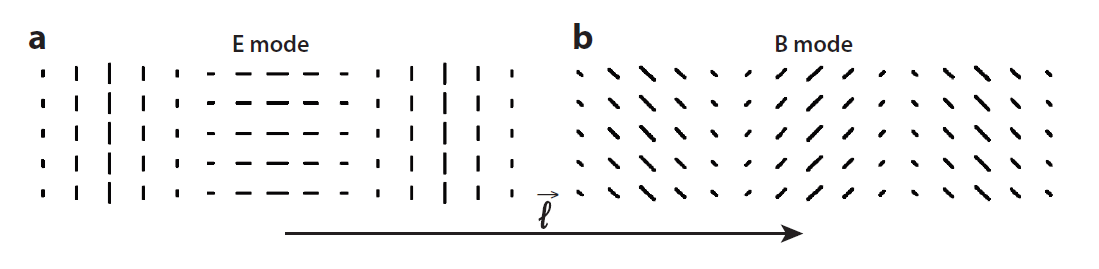
\includegraphics[width=0.7\linewidth]{EBintuition.png}
  \centering
  \caption{Polarization patterns associated with (a) a single E mode and (b) a single B mode with horizontal wavevector $\v{l}$. By C.Bischoff and taken from \cite{QBM}.}
  \label{EBint}
\end{figure}

\subsection{B Modes from IGWs}

Having discussed the relevant polarisation observables, we now wish to understand how they relate to our primordial inflationary spectra. The main goal of this section is to show that tensor perturbations source a non zero B mode polarisation, whose power spectrum depends on the primordial tensor power spectrum. We present the argument laid out in \cite{all-sky}, though see also \cite{kowosky} which rigorously derives the Boltzmann equations.\\

It is most convenient throughout to work in Fourier space with wave-vector $\v{k}$, and to rotate our coordinate system such that this is aligned with the $\unit{z}$ direction. There exist two independent polarisations of the tensor perturbation for our Fourier mode: $\xi^+$ and $\xi^\times$. We may choose simple polarisation vectors $e^+_{xx}=-e^+_{yy}=1$ and $e^\times_{xy}=e^\times_{yx}=1$ with all other components 0. In a cosmological context we take these modes to have equal amplitude i.e. $\xi^+(\v{k},\tau)=\xi^\times(\v{k},\tau)=h(\v{k},\tau)$. It is convenient to repackage them as
\begin{equation}
\xi^1 = (\xi^+ - i\xi^\times)/\sqrt{2} \qquad \xi^2 = (\xi^+ + i\xi^\times)/\sqrt{2}
\end{equation}

At $\tau=0$, inflation tells us $\xi^+$ and $\xi^\times$ are independent, and drawn from a Gaussian variate, whose individual power spectra are half of the total tensor power spectrum \ref{tensorpowerspec}. Our new variables, being linearly independent combinations of $\xi^s$, are also Gaussians, and a short calculation reveals they are also independent with each having also having half of the the total primordial tensor power, i.e. at $\tau=0$ 
\begin{equation}
\begin{split}
\langle \xi^{1*}(\v{k})\xi^{1}(\v{k'})\rangle=\langle \xi^{2*}(\v{k})\xi^{2}(\v{k'})\rangle &=\half (2\pi)^3\delta(\v{k}-\v{k'})P_t(k)\\
\langle \xi^{1*}(\v{k})\xi^{2}(\v{k'})\rangle &=0
\end{split}
\label{statprops}
\end{equation}

where $P_t(k) = \frac{2\pi^2}{k^3}\Delta_t^2(k)$ is the standard dimensionfull power spectrum. Note our fourier convention differs from \cite{all-sky}, who absorb the $(2\pi)^3$ into the power spectrum. This means our final angular power spectra will also differ by this factor.\\

To completely understand the full photon distribution we must follow the evolution of four distributions $f_X$, one for each Stokes parameter $X\in\{I,Q,U,V\}$. Thomson scattering of anisotropic radiation by free electrons gives rise to only linear polarization, so we may safely ignore $f_V$. For homogeneous and isotropic unpolarised radiation the distribution is simply $\bar{f}_I(\tau)= [e^{\hbar \nu/k_b T(\tau)}-1]^{-1}$, $f_Q=f_U=0$, the black body Planck distribution. The presence of metric perturbations breaks this homogeneity, inducing frequency independent perturbations $\Delta_X(\tau,\unit{n},\v{x})$ in real space or $\Delta_X(\tau,\unit{n},\v{k})$ in Fourier space.  Here, $\unit{n}$ is the line of sight, $\v{x}$ denotes spatial position, with conjugate $\v{k}$, and $\tau$ is conformal time. In principle these anisotropies additionally have frequency dependence, but since spectral distortions are second order we may ignore them at linear order. $Q$ and $U$ are measured in their natural basis ($\unit{e}_\theta, \unit{e}_\phi$) on the sphere, and the intensity anisotropy may be related to the temperature anisotropy via $\Delta_I/4=\Delta_T=\frac{\delta T}{\bar{T}}$. Following a method first introduced by Polnarev \cite{polnarev}, we introduce new variables $\tilde{\Delta}_T(\tau,\mu,k)$ and $\tilde{\Delta}_P(\tau,\mu,k)$ with simpler angular dependence to describe temperature and polarisation anisotropies, depending only on $\mu=\unit{n}\cdot\unit{k}=\cos\theta$ rather than on both $\theta$ and $\phi$. They are related to our original variables via
\begin{equation}\begin{split}
\Delta_T(\tau,\unit{n},\v{k}) &= [(1-\mu^2) e^{2i\phi} \xi^1(\v{k})+(1-\mu^2) e^{-2i\phi} \xi^2(\v{k})]\tilde{\Delta}_T(\tau,\mu,k)\\
(\Delta_Q+i\Delta_U)(\tau,\unit{n},\v{k}) &=[(1-\mu)^2 e^{2i\phi} \xi^1(\v{k})+(1+\mu)^2 e^{-2i\phi} \xi^2(\v{k})]\tilde{\Delta}_P(\tau,\mu,k) \\
(\Delta_Q-i\Delta_U)(\tau,\unit{n},\v{k}) &=[(1+\mu)^2 e^{2i\phi} \xi^1(\v{k})+(1-\mu)^2 e^{-2i\phi} \xi^2(\v{k})]\tilde{\Delta}_P(\tau,\mu,k)
\end{split}\end{equation}

and obey \textit{decoupled} Boltzmann equations, as derived in \cite{kowosky}, given by
\begin{equation}\begin{split}
\tilde{\Delta}_T'+ik\mu \tilde{\Delta}_T &= -h' -\kappa'[\tilde{\Delta}_T - \Psi]\\
\tilde{\Delta}_P'+ik\mu\tilde{\Delta}_P &= -\kappa'[\tilde{\Delta}_P + \Psi]
\end{split}
\label{Boltzmann}\end{equation}

where the source is
\begin{equation}
\Psi = \frac{1}{10}\tilde{\Delta}_{T0} + \frac{1}{7}\tilde{\Delta}_{T2} + \frac{3}{70}\tilde{\Delta}_{T4} - \frac{3}{5}\tilde{\Delta}_{P0} + \frac{6}{7}\tilde{\Delta}_{P2} - \frac{3}{70}\tilde{\Delta}_{P4}
\end{equation}

written in terms of moments, given by $\Delta(k, \mu) = \sum_l (2l+1)(-i)^l\Delta_l(k)P_l(\mu)$ for $P_l(\mu)$ the order $l$ Legendre polynomial. All derivatives are taken with respect to conformal time $\tau$. $h$ is the gravitational wave amplitude. $\kappa$ is the Thomson optical depth, described in more detail in the next section. These equations encode relatively simple physics. The left hand sides are simply the Lagrangian time derivatives of a Fourier mode with wave number $k$. The $h'$ in the first equation encodes the temperature variation induced by the gravitational wave. While not present explicitly in the polarisation equation, it also affects it through the source term $\Psi$, which depends on moments of the temperature fluctuation. The terms multiplying $\kappa'$ come from the Thomson scattering collision term of the Boltzmann equation, and are derived using the angular dependence of the Thomson differential cross section from QED \cite{QBM, kowosky}. \\

By multiplying the Boltzmann equations \ref{Boltzmann} by $P_l(\mu)$ and integrating over angular dependence $\mu$, making use of the relevant identities for Legendre polynomials, we obtain a heirachy of equations connecting higher moments to lower, a fact we will use later.

\subsubsection{Recombination History}

While the Universe is young and hot, baryons are ionised and tightly coupled to photons via Thomson scattering. Once the temperature falls below a few eV, it becomes favourable for electrons and ions to recombine to form neutral molecules. As the number of charged particles falls, the mean free path of any given photon increases. Eventually, the mean free path becomes comparable to the horizon size and the photon and baryon fluids are essentially decoupled. It is at this point in the Universe’s evolution that the CMB photons last scatter \cite{Pritchard}.\\

The visibility function describes the probability density that a given CMB photon last scattered at a particular $\tau$. It is given terms of the optical depth $\kappa$ as
\begin{equation}
g(\tau) = -\kappa'e^{-\kappa}
\label{RH1}
\end{equation}

where $\kappa' = an_ex_e\sigma_T$ is the differential optical depth, the scale factor multiplied by the electron number density, ionisation fraction, and Thomson cross section. The optical depth between conformal time $\tau$ and today is given by the integral of this 
\begin{equation}
\kappa(\tau) = \int_\tau^{\tau_0} \kappa'(\tau')d\tau'
\end{equation}

with limiting values $\kappa(\tau_0) = 0$ and $\kappa(0)\rightarrow \infty$ today and in the far past. Numerical calculations show that $g(\tau)$ is sharply peaked around recombination. The simplest approximation takes it to be a delta function, and bears the name `instantaneous recombination', as every photon decouples at the same time. The next simplest approximation is to take the visibility function to be a narrow Gaussian
\begin{equation}
g(\tau) = g(\tau_R)e^{-\frac{(\tau-\tau_R)^2}{2\Delta\tau_R^2}}
\label{RH2}
\end{equation}

where $\tau_R$ is the time of recombination, $\Delta\tau_R$ is its width, and $g(\tau_R)$ is the amplitude. We will also make use of an approximation for the optical depth during recombination. Writing $\kappa = e^{-f(\tau)}$, consistency between \ref{RH1} and \ref{RH2} requires $\kappa \approx e^{-(\tau-\tau_R) / \Delta\tau_R}$ and $g(\tau_R)\approx 1/(e\Delta\tau_R)$ near $\tau_R$. 

\begin{figure}[h]
  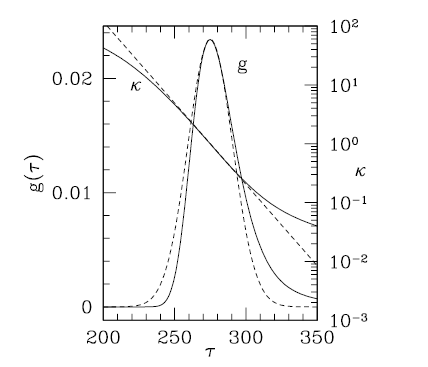
\includegraphics[width=0.5\linewidth]{recombinationhistory.png}
  \centering
  \caption{Recombination history. Plotted are the visibility function and optical depth calculated numerically in bold, and the Gaussian approximation with $\Delta\tau_R=15.7$, dashed. }
\end{figure}

This is a decent approximation but we find it isn't quite right. In particular, after the `dark ages' in which the universe is very neutral, we know from observations of quasar absorption spectra that the universe is highly ionized again at $5<z<20$. This reionization is driven by radiation from the first stars interacting with hot hydrogen gas. CMB photons therefore enter a second phase of Thomson scattering at a later time \cite{reionisation}, which is important to account for in our CMB theory.

\subsubsection{Line of Sight Expressions}

While one may solve the boltzmann heirachy directly from initial conditions, it proves more instructive and intuitive to use the `line of sight method', first introduced in \citep{LoS}. We formally integrate these first order linear ODEs, making use of an integrating factor $e^{ik\mu\tau+\kappa}$, from their initial conditions up until today.  Introducing $x=k(\tau_0-\tau)$ we get  
\begin{equation}\begin{split}
\tilde{\Delta}_T(\tau_0,\mu,k) &= \int_0^{\tau_0}d\tau e^{-ix\mu}S_T(k,\tau)\\
\tilde{\Delta}_P(\tau_0,\mu,k) &= \int_0^{\tau_0}d\tau e^{-ix\mu}S_P(k,\tau)
\end{split}\end{equation}

after multiplying by the integrating factor, integrating, making use of $\kappa(\tau_0)=0$ and $\kappa(0)\rightarrow \infty$ to evaluate the left hand side limits, and finally dividing through by $e^{ik\mu\tau_0}$. All the physics is hidden in the source terms
\begin{equation}\begin{split}
S_T(k,\tau) &= -h'e^{-\kappa}+g\Psi\\
S_P(k,\tau) &= -g\Psi
\end{split}\end{equation}

which we'll explore in \ref{interpretation}. This let's us write
\begin{equation}\begin{split}
\Delta_T(\tau_0,\unit{n},\v{k}) &= [(1-\mu^2) e^{2i\phi} \xi^1(\v{k})+(1-\mu^2) e^{-2i\phi} \xi^2(\v{k})]\int_0^{\tau_0}d\tau e^{-ix\mu}S_T(k,\tau)\\
(\Delta_Q+i\Delta_U)(\tau_0,\unit{n},\v{k}) &=[(1-\mu)^2 e^{2i\phi} \xi^1(\v{k})+(1+\mu)^2 e^{-2i\phi} \xi^2(\v{k})]\int_0^{\tau_0}d\tau e^{-ix\mu}S_P(k,\tau)\\
(\Delta_Q-i\Delta_U)(\tau_0,\unit{n},\v{k}) &=[(1+\mu)^2 e^{2i\phi} \xi^1(\v{k})+(1-\mu)^2 e^{-2i\phi} \xi^2(\v{k})]\int_0^{\tau_0}d\tau e^{-ix\mu}S_P(k,\tau)
\end{split}\end{equation}

The T result is what we want. Recall Q and U however are coordinate dependent quantities on the sphere, which are a nuisance. We work instead with $\tilde{E}$ and $\tilde{B}$. \ref{EBmodes} tells us to convert between them all we need to do is act twice via our raising and lowering operators. We make use of \ref{+-2}, which conveniently pass through the source terms, which have no angular dependence, arriving at
\begin{equation}\begin{split}
\sl^2(\Delta_Q+i\Delta_U)(\tau_0,\unit{n},\v{k}) &= \xi^1(\v{k})e^{2i\phi}\int_0^{\tau_0}d\tau S_P(k,\tau)(-\partial_\mu+\frac{2}{1-\mu^2})^2[(1-\mu^2)(1-\mu)^2 e^{-ix\mu}]\\
&\quad + \xi^2(\v{k})e^{-2i\phi}\int_0^{\tau_0}d\tau S_P(k,\tau)(-\partial_\mu-\frac{2}{1-\mu^2})^2[(1-\mu^2)(1+\mu)^2 e^{-ix\mu}]\\
&= -\xi^1(\v{k})e^{2i\phi}\int_0^{\tau_0}d\tau S_P(k,\tau)(\hat{\mathcal{E}}(x)-i\hat{\mathcal{B}}(x))[(1-\mu^2) e^-{ix\mu}] \\
&\quad - \xi^2(\v{k})e^{-2i\phi}\int_0^{\tau_0}d\tau S_P(k,\tau)(\hat{\mathcal{E}}(x)+i\hat{\mathcal{B}}(x))[(1-\mu^2) e^{-ix\mu}] 
\end{split}\end{equation}
\begin{equation}\begin{split}
\sr^2(\Delta_Q-i\Delta_U)(\tau_0,\unit{n},\v{k}) &= \xi^1(\v{k})e^{2i\phi}\int_0^{\tau_0}d\tau S_P(k,\tau)(-\partial_\mu-\frac{2}{1-\mu^2})^2[(1-\mu^2)(1+\mu)^2 e^{-ix\mu}] \\ 
&\quad + \xi^2(\v{k})e^{-2i\phi}\int_0^{\tau_0}d\tau S_P(k,\tau)(-\partial_\mu+\frac{2}{1-\mu^2})^2[(1-\mu^2)(1-\mu)^2 e^{-ix\mu}]\\
&= -\xi^1(\v{k})e^{2i\phi}\int_0^{\tau_0}d\tau S_P(k,\tau)(\hat{\mathcal{E}}(x)+i\hat{\mathcal{B}}(x))[(1-\mu^2) e^{-ix\mu}] \\
&\quad - \xi^2(\v{k})e^{-2i\phi}\int_0^{\tau_0}d\tau S_P(k,\tau)(\hat{\mathcal{E}}(x)-i\hat{\mathcal{B}}(x))[(1-\mu^2) e^{-ix\mu}] 
\end{split}\end{equation}

where we have introduced differential operators, which will save us some work very soon.
\begin{equation}
\hat{\mathcal{E}}(x)=-12+x^2(1-\partial^2_x)-8x\partial_x \qquad \mathcal{\hat{B}}(x) = 8x+2x^2\partial_x
\end{equation}

Plugging these into \ref{EBmodes} we find our final results for each Fourier mode to be
\begin{equation}\begin{split}
\Delta_T(\tau_0,\unit{n},\v{k}) &= [(1-\mu^2) e^{2i\phi} \xi^1(\v{k})+(1-\mu^2) e^{-2i\phi} \xi^2(\v{k})]\int_0^{\tau_0}d\tau e^{-ix\mu}S_T(k,\tau)\\
\Delta_{\tilde{E}}(\tau_0,\unit{n},\v{k}) &= [(1-\mu^2) e^{2i\phi} \xi^1(\v{k})+(1-\mu^2) e^{-2i\phi} \xi^2(\v{k})]\hat{\mathcal{E}}(x)\int_0^{\tau_0}d\tau e^{-ix\mu}S_P(k,\tau)\\
\Delta_{\tilde{B}}(\tau_0,\unit{n},\v{k}) &= [(1-\mu^2) e^{2i\phi} \xi^1(\v{k})+(1-\mu^2) e^{-2i\phi} \xi^2(\v{k})]\hat{\mathcal{B}}(x)\int_0^{\tau_0}d\tau e^{-ix\mu}S_P(k,\tau)
\label{LoSFourier}
\end{split}\end{equation}

The complete solution requires integration over all Fourier modes, which evolve independently. Note the phase factor vanishes as we evaluate all terms at the same spatial position $\v{x}=0$ 
\begin{equation}\begin{split}
\Delta_T(\tau_0,\unit{n}) &= \fint{k} \Delta_T(\tau_0,\unit{n},\v{k})\\
\Delta_{\tilde{E}}(\tau_0,\unit{n}) &= \fint{k} \Delta_{\tilde{E}}(\tau_0,\unit{n},\v{k})\\
\Delta_{\tilde{B}}(\tau_0,\unit{n}) &= \fint{k} \Delta_{\tilde{B}}(\tau_0,\unit{n},\v{k})
\end{split}\end{equation}

If we had chosen to work with Q and U here, in order to sum up Fourier modes with respect to a fixed basis with respect to the sphere, we would need to rotate each $Q\pm iU$ $\v{k}$ mode by a $\v{k}$ and $\unit{n}$ dependent phase (since we aligned $\v{k}$ with $\unit{z}$). This was a complication in early attempts to characterise the CMB polarisation beyond the flat sky regime, and we have avoided it through our definition of rotationally invariant E and B modes.\\

We see tensor perturbations have induced both E and B modes.

\subsubsection{Tensor Power Spectra}

Thankfully the form of these are very similar, allowing us to compute all the power spectra in one go. We'll begin by calculating the TT power spectrum $C_l^{TT}$ sourced by tensor perturbations. Using the expression for spherical multipole coefficients 

\begin{equation}
T_{lm} = \int d\Omega Y_{lm}^*(\unit{n})\Delta_T(\tau_0,\unit{n})
\end{equation}

and making use of \ref{powerspectra} we can write 
\begin{equation}\begin{split}
C_l^{TT} &= \frac{1}{2l+1}\sum_m \langle T_{lm}^*T_{lm} \rangle \\
&\supset \frac{4\pi}{2l+1} \int k^2 dk \frac{P_t(k)}{2} \sum_m \bigg| \int d\Omega Y^*_{lm}(\unit{n}) \int_0^{\tau_0} d\tau  S_T(k,\tau)(1-\mu^2)e^{2i\phi}e^{-ix\mu} \bigg|^2\\
&= 2\pi^2\ltwof \int k^2 dk P_t(k) \bigg|  \int_0^{\tau_0} d\tau  S_T(k,\tau)\int_{-1}^1 d\mu P_l^2(\mu)(1-\mu^2)e^{-ix\mu} \bigg|^2\\
&= 2\pi^2\ltwof \int k^2 dk P_t(k) \bigg|  \int_0^{\tau_0} d\tau  S_T(k,\tau)\int_{-1}^1 d\mu \partial_\mu^2P_l(\mu)(1-\mu^2)^2e^{-ix\mu}\bigg|^2\\
&= 2\pi^2\ltwof \int k^2 dk P_t(k) \bigg|  \int_0^{\tau_0} d\tau  S_T(k,\tau)\int_{-1}^1 d\mu \partial_\mu^2P_l(\mu)(1+\partial_x^2)^2e^{-ix\mu} \bigg|^2\\
&= 2\pi^2\ltwof \int k^2 dk P_t(k) \bigg|  \int_0^{\tau_0} d\tau  S_T(k,\tau)\int_{-1}^1 d\mu P_l(\mu)(1+\partial_x^2)^2(x^2e^{-ix\mu}) \bigg|^2\\
&= 2\pi^2\ltwof \int k^2 dk P_t(k) \bigg|  \int_0^{\tau_0} d\tau  S_T(k,\tau)(1+\partial_x^2)^2\left(x^2 \int_{-1}^1 d\mu P_l(\mu)e^{-ix\mu} \right)\bigg|^2\\
&= 8\pi^2\ltwof \int k^2 dk P_t(k) \bigg|  \int_0^{\tau_0} d\tau  S_T(k,\tau) (1+\partial_x^2)^2\left(x^2j_l(x)) \right)\bigg|^2\\
&= 8\pi^2\ltwo \int k^2 dk P_t(k) \bigg|  \int_0^{\tau_0} d\tau  S_T(k,\tau)\frac{j_l(x)}{x^2} \bigg|^2\\
\end{split}\end{equation}

Where we have used the statistical properties \ref{statprops} of $\xi^i(\v{k})$ to compute the primordial expectation value. For readability we have only included the piece arising from $\xi^1$. The piece arising from $\xi^2$ differs in the second line by replacing $e^{2i\phi}$ with its complex conjugate $e^{-2i\phi}$, and can easily be shown to contribute exactly the same, using properties of $P_l^m$ (omitted). The power spectra is therefore twice the result above.\\

To evaluate the angular integrals, we used the expression for spherical harmonics in terms of legendre polynomials.
\begin{equation}
Y_{lm} = \left[\frac{(2l+1)(l-m)!}{4\pi(l+m)!}\right]^\half P_l^m(\mu)e^{-im\phi}
\end{equation}
The $\phi$ integral vanishes unless $m=2$, in which case it gives $2\pi$. Then, for the $\mu$ integral we make use of 
\begin{equation}
P^m_l(\mu)=(-1)^m(1-\mu^2)^{m/2}(\partial_\mu)^mP_l(\mu)
\end{equation}
and integrate by parts twice giving the factor of $x^2$. Then we use 
\begin{equation}
\int_{-1}^1 d\mu e^{-ix\mu}P_l(\mu) = 2(-i)^lj_l(x)
\end{equation}
to perform the $\mu$ integral. Finally we make use of the differential equation
\begin{equation}
j_l''+\frac{2j_l'}{x}+\left(1-\frac{l(l+1)}{x^2}\right)j_l=0
\end{equation}
to eliminate derivatives of bessel functions and obtain
\begin{equation}
(1+\partial_x^2)^2[x^2j_l(x)] = (l-1)l(l+1)(l+1)\frac{j_l}{x^2}
\end{equation}
explaining the change in the $l$ dependent prefactor in the last line.\\

This gives final result for the temperature power spectrum. Now we abuse the similarity of expressions in \ref{LoSFourier} to write down the EE and BB power spectra. The angular dependence of $\Delta_{\tilde{E}}$ and $\Delta_{\tilde{B}}$ are exactly the same as those of $\Delta_T$, with the expressions only differing in the operators $\hat{\mathcal{E}}$ and $\hat{\mathcal{B}}$, acting seperately on each $\v{k}$ mode, which can be applied after the angular integrals are performed. We lose the $l$ dependent factor in front by converting from $\tilde{E}, \tilde{B}$ to $E,B$, using \ref{EBmodes}
\begin{equation}\begin{split}
C_l^{EE} &= (4\pi)^2 \int k^2 dk P_t(k) \bigg|  \int_0^{\tau_0}d\tau  S_P(k,\tau)\hat{\mathcal{E}}(x)\frac{j_l(x)}{x^2} \bigg|^2\\
&= (4\pi)^2\int k^2 dk P_t(k) \bigg|  \int_0^{\tau_0}d\tau  S_P(k,\tau)[-j_l(x) +j_l''(x)+\frac{2j_l(x)}{x^2} + \frac{4j_l'(x)}{x}]\bigg|^2\\
C_l^{BB} &= (4\pi)^2 \int k^2 dk P_t(k) \bigg|  \int_0^{\tau_0}d\tau  S_P(k,\tau)\hat{\mathcal{B}}(x)\frac{j_l(x)}{x^2} \bigg|^2\\
&= (4\pi)^2\int k^2 dk P_t(k) \bigg|  \int_0^{\tau_0} d\tau S_P(k,\tau)[2j_l'(x)+\frac{4j_l(x)}{x}]\bigg|^2
\label{primordialBmodes}
\end{split}\end{equation}

Having computed these, we may repackage these power spectra neatly by reading off the multipole moments due to a single wave number k as 
\begin{equation}
\begin{split}
\Delta_{Tl}(k) &= \ltwo^\half \int_0^{\tau_0} d\tau \left(-h'(\tau)e^{-\kappa(\tau)}-g(\tau)\Psi(k,\tau)\right)\frac{j_l(x)}{x^2}\\
\Delta_{El}(k) &= \int_0^{\tau_0}d\tau  \left(-g(\tau)\Psi(k,\tau)\right)\left[-j_l(x) +j_l''(x)+\frac{2j_l(x)}{x^2} + \frac{4j_l'(x)}{x}\right]\\
\Delta_{Bl}(k) &= \int_0^{\tau_0} d\tau \left(-g(\tau)\Psi(k,\tau)\right)\left[2j_l'(x)+\frac{4j_l(x)}{x}\right]
\end{split}
\end{equation}
 
with $x=k(\tau_0-\tau)$. These may be further integrated by parts to improve computational efficiency by moving derivatives off the bessel functions. Power spectra may be written in terms of these as 

\begin{equation}
C_l^{XY} = (4\pi)^2 \int k^2 dk P_t(k) \Delta_{Xl}(k)\Delta_{Yl}(k)
\end{equation}

which are non vanishing only for $XY \in \{TE, TT, EE, BB\}$. 

\subsection{Interpretation of Power Spectra}
\label{interpretation}

Having written down expressions for the power spectra contributions of tensor modes we now wish to understand what they look like. As seen when studying CMB anistropies, it is possible to get a good qualitative understanding for the shape of power spectra working analytically, though when percent level precision is needed a suitable numerical code must be used.\\

To do so, we need to understand the objects in the main results above. We have already discussed the visibility function $g$. All power spectra also depend on the unknown tensor power spectrum, which controls their overall amplitude, and also affects their scale dependence. For figures, we take  $A_t = \frac{1}{8(4\pi)^2}, n_t=0$, and remaining cosmological parameters to be a $\Lambda$CDM cosmology with $\Omega_b=0.05, \Omega_{DM}=0.25, \Omega_\Lambda=0.7$ and Hubble parameter $h=0.72$. This sections discussion and figures are in large part from \cite{Pritchard}, though also see \cite{zhao}. It remains to discuss the gravitational wave amplitude evolution $h'$, the projection functions, and finally the source term $\Psi$, a function of polarisation and temperature anisotropy moments. First however we give some intuition about the expected shape of power spectra, shown in figure \ref{tensorpower}.

\begin{figure}[h]
  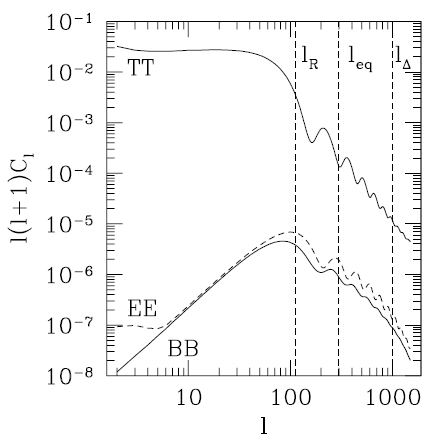
\includegraphics[width=0.5\linewidth]{tensorpowerspectra.png}
  \centering
  \caption{Tensor power spectra, with vertical lines indicating the three important angular scales, horizon size at recombination $\tau_R$, horizon size at matter-radiation equality $\tau_{eq}$ and width of last-scattering surface $\Delta\tau_R$}
  \label{tensorpower}
\end{figure}


Temperature anisotropies 
\begin{equation}
\Delta_{Tl} = \ltwo^\half \int_0^{\tau_0} d\tau (-h'e^{-\kappa}+g\Psi)\frac{j_l(x)}{x^2}\\
\end{equation}

have two contributions. The second source term is localised at the surface of last scattering (SLS) by the visibility function, and will be discussed in some detail below. It turns out to be subleading at all scales. The first is a form of integrated Sachs-Wolfe term, describing the anisotropy generated by the photon travelling through a changing gravitational potential on its path to us. Between the SLS and today, the average amplitude of the gravitational wave decreases (as it is redshifted), and so the mean energy of photon increases. Today, the gravitational wave background is negligible, and as a result, the final energy of photon is determined by whether its journey from the SLS started in a trough or crest of the tensor mode. Akin to the usual ISW effect, this term is responsible for the large scale flat nature of the TT power spectrum.\\


Polarisation anisotropies can be written
\begin{equation}
\Delta_{Xl} = \int_0^{\tau_0} d\tau (-g\Psi) P_{Xl}(k(\tau_0-\tau))\\
\end{equation}

involving a single SLS localised source, and an $l$ dependent projection function. This is sensible, as free streaming photons, while experiencing energy shifts due to cosmic expansion, should not be repolarised after last scattering. Considering photons scattering off an electron in its rest frame arrive from all directions from a mean distance determined by the mean free path at recombination. During propagation, they experience the ISW effect, discussed above, and so arrive with different temperatures, i.e. we have a temperature quadrupole which after scattering rise to linear polarisation. \\

The power spectrum can be understood as follows. By causality, the gravitational wave amplitude is constant on super horizon scales, but, like radiation, we expect it to decay rapidly upon entering the horizon. So, photons incident on modes that are super horizon at last scattering don't experience much ISW temperature change and generate little polarisation. Optimal ISW and thus maximal polarisation is generated by modes entering the horizon at the time of penultimate scattering, as this is the period in which the gravitational wave loses most of its amplitude. Translating into the form of the polarisation power spectrum, we expect to see a slow increase in power at large scales, peaking at the horizon scale at penultimate scattering. For smaller scales we expect a drop corresponding to the transition between modes entering in the penultimate to last scattering period and those not. The matter-radiation equality scale should be distinctive due to it the gravitational wave amplitude exhibiting differing scaling in the two eras. On very small scales, phase cancellation, defined later but resulting in a similar effect to diffusion damping, becomes important and leads to an exponential suppression. 

\subsubsection{Gravitational Wave Evolution}
\label{evolution}

Gravitational waves frozen after inflation become dynamical upon horizon reentry, with amplitude sources temperature fluctuations in the CMB. Their evolution is determined by the Einstein equation, given by \cite{Pritchard}

\begin{equation}
h_{ij}''+2\mathcal{H}h_{ij}'-\nabla^2h_{ij} = 16\pi Ga^2\Pi_{ij}
\end{equation}

where $\Pi_{ij}$ is the anisotropic stress, sourced in small amounts by neutrino free-streaming. In the absence of anisotropic stress, and decomposing the tensor perturbation into its polarisation states in Fourier space we find each of $h_+$ and $h_\times$ satisfy

\begin{equation}
h''+2\mathcal{H}h'+k^2h = 0
\end{equation}

which one can equivalently obtain by recalling each mode of the tensor perturbation $ah_\v{k}$ obeys the Muhkanov-Sasaki equation \ref{MS}.  Of particular interest is the matter dominated era where $\mathcal{H}=2/\tau$. Upon performing the change of variable $x=k\tau,  h=f(x)/x$ we obtain
\begin{equation}
x^2\frac{d^2f}{dx^2}+2x\frac{df}{dx}+(x^2-2)f=0
\end{equation}

which we recognise as the $l=1$ spherical bessel equation, with regular solution $f(x) = j_1(x)$. We therefore have
\begin{equation}
h^{\text{mat}}_\v{k}(\tau) = 3h_\v{k}(0)\frac{j_1(k\tau)}{k\tau}
\end{equation}

The relevant quantity is the conformal time derivative of this, which we may obtain using the property
\begin{equation}
j_{n+1}(x)=-(-x)^n\frac{d}{dx}(-x)^{-n}j_n(x)
\end{equation}

leading to 
\begin{equation}
h^{\text{mat}'}_\v{k}(\tau) = -3h_\v{k}(0)\frac{j_2(k\tau)}{\tau}
\end{equation}

A similar method can be applied to the radiation dominated epoch, with $\mathcal{H}=1/\tau$, to obtain
\begin{equation}
h^{\text{rad}}_\v{k}(\tau) = h_\v{k}(0)j_0({k\tau})
\end{equation}

The behaviour of these solutions splits into three regimes. When $k\tau\ll 1$, $h$ evolves slowly and is approximately constant, corresponding to a frozen superhorizon mode. For $k\tau\approx1$, the amplitude decays rapidly and settles into an oscillatory phase with decaying amplitude for $k\tau \gg 1$, corresponding to the mode enetering the horizon and redshifting away. See figure \ref{gravwave}. Since recombination occurs shortly after matter domination, we expect the form $h^{\text{mat}}$ to be a good description for modes entering the horizon during matter domination, though for modes entering during radiation domination we expect the radiation to matter domination transition to affect evolution significantly.\\

\begin{figure}[h]
  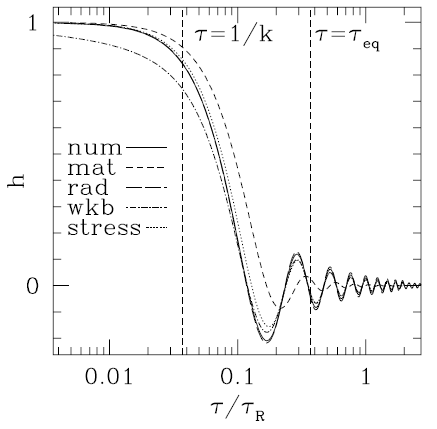
\includegraphics[width=0.5\linewidth]{gravwaveev.png}
  \centering
  \caption{Gravitational wave evolution at wavenumber satisfying $k\tau_{eq}=10$. Shown solutions are numerical without anisotropic stress, analytic matter domination, analytic radiation domination, a WKB approximation, and numerical with anisotropic stress}
  \label{gravwave}
\end{figure}

Even without a complete analytical solution, we may obtain the scaling of $h$ via a simple argument. Before horizon entry,  by causality the amplitude $h$ should be constant. After horizon entry, the gravitational wave redshifts with expansion as radiation (the graviton is massless), and scales as $h\sim 1/a$. Hence we have the relation between the gravitational wave amplitude today and at horizon entry $h_{\text{today}}/h_{\text{entry}} = a_{\text{today}}/a_{\text{entry}}$. Taking $h_{\text{entry}}$ to be independent of $k$, we have $h_{\text{today}}\propto a_{\text{entry}}$. Horizon entry occurs when $a_{\text{entry}}H_{\text{entry}}=k$ and so from the scaling of H in matter and radiation domination we obtain $a_{\text{entry}}\propto k^{-1}$ for radiation domination and $a_{\text{entry}}\propto k^{-2}$ for matter domination. This gives the scalings

\begin{equation}
  h \propto
    \begin{cases}
      1 & k<1/\tau_0\\
      k^{-2} & 1/\tau_0<k<1/\tau_{eq}\\
      k^{-1} & 1/\tau_{eq}<k
    \end{cases}       
\end{equation}

For polarisation $X\in\{E,B\}$ we therefore expect since $k\sim l$ and $C_l^{XX}\sim (h')^2$ that

\begin{equation}
  l(l+1)C_l^{XX} \propto
    \begin{cases}
      l^2 & l<l_R\\
      l^{-2} & l_R<l<l_{eq}\\
      l^{-4} & l_{eq}<l
    \end{cases}       
\end{equation}

which can be seen in the power spectra, clearly demonstrating the peak at $l_R$ and the different scalings for modes entering in matter and radiation domination.


\subsubsection{Projection Factors}

When viewing the CMB we are viewing the projection of a 3D system onto a sphere. We can think of the weird looking spherical bessel like terms as projection factors, defining
\begin{align}
P_{Tl}(x) &= \frac{j_l(x)}{x^2}\\
P_{El}(x) &= -j_l(x) +j_l''(x)+\frac{2j_l(x)}{x^2} + \frac{4j_l'(x)}{x}\\
P_{Bl}(x) &= 2j_l'(x)+\frac{4j_l(x)}{x}
\end{align}

with argument $x=k(\tau_0-\tau)$, the lookback time scaled by wavenumber. 

\begin{figure}[h]
  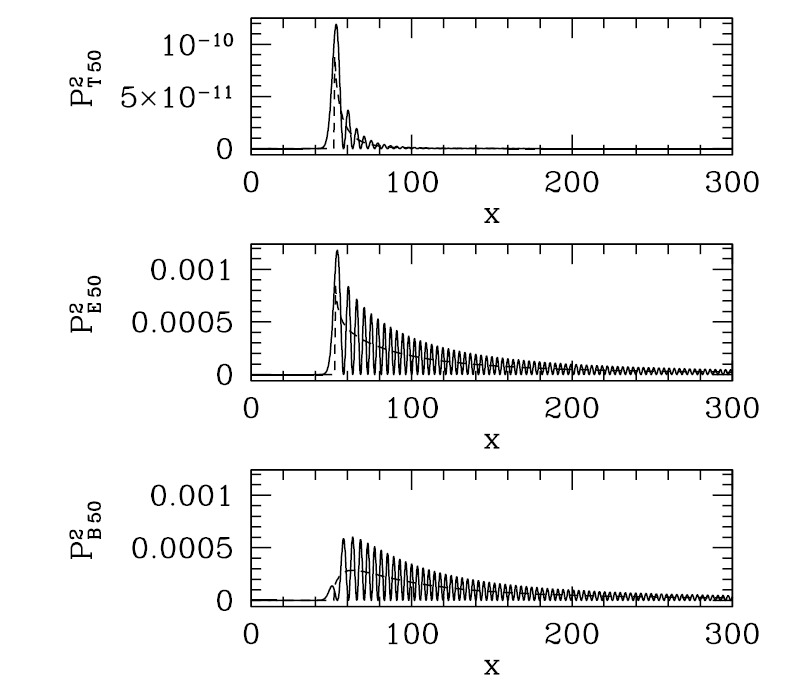
\includegraphics[width=0.7\linewidth]{projection.png}
  \label{proj}
  \centering
  \caption{Squares of projection terms for $l=50$. Dashed curve shows time averaged analytic approximations used.}
\end{figure}


These are all peaked at $x\approx l$, i.e. $C_l$ is dominated by the behaviour of the source at $x\approx l$. The polarisation source function is strongly peaked at $\tau=\tau_R$, implying $k\approx l/(\tau_0-\tau_R)$ dominates the power spectrum. The departure of these projectors from a delta function, ie the large $x>l$ tail, indicates larger wave number modes also contribute to power at this angular scale, giving an overall smoothing to the power spectrum.\\

There exist several approximations for spherical bessel functions at $x\gg l$ and $x\ll l$, but unfortunately for our purposes we are interested in the peaks at $x\approx l$. Noticing the projection functions only really contribute for $x>l$ we may use the approximation valid for $x>l$

\begin{equation}
j_l(x) = \frac{1}{\sqrt{x^2\sin\alpha}}\cos[x(\sin\alpha-\alpha\cos\alpha)-\pi/4]
\end{equation}

with $\cos\alpha=(l+1/2)/x$. This reduces to the more familiar $j_l(x) \approx \sin(x-l\pi/2)/x$ for $x\gg l$. In power spectra, these projection functions will appear as squares, and their fast time oscillations aren't important. We may therefore time average, making use of the relations $\langle \sin^2x \rangle = \langle \cos^2x \rangle = 1/2$ and $\langle \sin x\cos x \rangle = 0$ to obtain explicit expressions. For instance,

\begin{equation}
\langle P_T(x)^2 \rangle \approx \frac{1}{2x^5\sqrt{x^2-l^2}}
\end{equation}

with similar more complicated expressions for E, B (plotted in figure \ref{proj}). Note these diverge as $x\rightarrow l$, and so we must introduce an order unity cut-off $a$ and restrict to the domain $x>l+a$





\subsubsection{Source Evolution}

One begins by expanding the Boltzmann equation \ref{Boltzmann} into an infinite `heirachy' of moments. These may be numerically integrated time-step by time-step, up to some arbitrary large cut off $l$, which is the approach taken by codes. To make analytical progress, we employ the tight coupling approximation, in which higher order moments are suppressed by the scattering rate, $\kappa'$ being large during recombination. Each moment is smaller than the last by a factor of of $\kappa'$, and so to leading order we may keep just	
\begin{equation}
\begin{split}
\tilde{\Delta}_{T0}'&=-h'-\kappa'[\tilde{\Delta}_{T0}-\Psi]\\
\tilde{\Delta}_{P0}'&=-\kappa'[\tilde{\Delta}_{T0}+\Psi]\\
\tilde{\Delta}_{Tl}'&=0\quad\text{for} \quad l\geq1\\
\tilde{\Delta}_{Pl}'&=0\quad\text{for} \quad l\geq1
\end{split}
\end{equation}
In this limit $\Psi = \frac{1}{10}\tilde{\Delta}_{T0} - \frac{3}{5}\tilde{\Delta}_{P0}$, and so combining the first two equations we obtain
\begin{equation}
\Psi ' +\frac{3}{10}\kappa'\Psi = -\frac{h'}{10}
\end{equation}

Employing the line of sight method once more we obtain

\begin{equation}
\Psi(\tau) = -\int_0^\tau d\tau' \frac{h'(\tau')}{10}\exp{\left( -\frac{3}{10}(\kappa(\tau')-\kappa(\tau))\right)}
\end{equation}

Now making the previously Gaussian approximation on the visibility function \ref{RH2} we take $\kappa'\approx -\kappa/\Delta\tau_R$. Changing variable of integration to $x=\kappa(\tau')/\kappa(\tau)$ gives

\begin{equation}
\Psi(\tau) = -\frac{h'(\tau_R)}{10}e^{3\kappa(\tau)/10}\Delta\tau_R\int_1^\infty\frac{dx}{x}e^{-3\kappa x/10}
\end{equation}

In pulling the gravitational wave amplitude out of the integral we have assumed $h$ varies slowly over the visibility function, an assumption only valid for modes $k\ll 1/\Delta\tau_R$. At larger wavenumbers $h$ oscillates rapidly over the visibility function and so we may improve this by replacing $h'(\tau_R)$ with its time averaged value over the visibility function

\begin{equation}
\langle h'(\tau) \rangle = \int_0^{\tau} d\tau' g(\tau')h'(\tau') \approx h'(\tau_R)e^{-(k\Delta\tau_R)^2/2}
\end{equation}

obtained through treating $h'$ as purely oscillatory with a slowly varying envelope. Integrating an oscillatory function over a Gaussian leads to the function evaluated at its peak multiplied by an exponential suppression. We see a small scale damping effect, akin to the diffusion damping encountered when considering scalar perturbations. In this context we term this phase damping - large k modes have contributions from many different regions in the SLS, each with a different phase. The net result is cancellation and a decrease and smoothing in observed power.\\

\subsubsection{Analytic Power Spectra}

Armed with an analytic solution for $\Psi$ we proceed to compute the polarisation multipole generated. For $X\in\{E,B\}$ we have
\begin{equation}
\begin{split}
\Delta_{Xl} &= \int_0^{\tau_0} d\tau [-g\Psi P_{Xl}(k(\tau_0-\tau))]\\
&\approx P_{Xl}(k(\tau_0-\tau_R)) \int_0^{\tau_0} d\tau [-g\Psi] \\
&= P_{Xl}(k(\tau_0-\tau_R)) \frac{h'(\tau_R)}{10}\Delta\tau_Re^{-(k\Delta\tau_R)^2/2} \int_0^\infty d\kappa e^{-7\kappa/10} \int_1^\infty\frac{dx}{x}e^{-3\kappa x/10}\\
&=P_{Xl}(k(\tau_0-\tau_R)) h'(\tau_R)\Delta\tau_Re^{-(k\Delta\tau_R)^2/2} (\frac{1}{7}\log{\frac{10}{3}})
\end{split}
\end{equation}

where, in the second line we pull the projection term outside the integral, assuming it varies slowly over the width of the visibility function. In the third line we convert from a conformal time to optical depth integral, and in the last line we have evaluated the integrals to $(10/7)\log{10/7}$. From this we may calculate the polarisation power spectra
\begin{equation}
C_l^{XY} = (4\pi)^2 (\frac{1}{7}\log{\frac{10}{3}})^2 \int k^2dk P_t(k) P_{Xl}(k(\tau_0-\tau_R))P_{Yl}(k(\tau_0-\tau_R))h'(\tau_R)^2(\Delta\tau_R)^2e^{-(k\Delta\tau_R)^2}
\end{equation}

We have analytic solutions to all of these quantities, which we proceed to plot in figure \ref{analytic1}. For the B mode spectra of interest, we see the analytic solution is rather good for low l, the regime in which our assumptions are most valid. The key features of the spectrum are as follows. We have a peak at $l\approx 90$, corresponding to the horizon size at penultimate scattering. Analytically, this is firstly due to the projection terms being combinations of bessel functions $j_l(k(\tau_0-\tau_R))$ peaking at $l\approx k(\tau_0-\tau_R)\approx k\tau_0$. Then recalling in matter domination $h'(\tau_R) \sim \frac{j_2(k\tau_R)}{\tau_R}$, and using that $j_2(x)$ peaks at $x\approx3$ we see a peak of $h'$ at $k\tau_R=3$, and so overall we have a peak at $l\approx k\tau_0\approx 3\tau_0/\tau_R$. The height of this peak is controlled both by $r$, giving the amplitude of $h$, but also by the duration of last scattering, through the $\Delta\tau_R$ term. We get further peaks, due to the oscillatory behaviour seen in the evolution of $h$, which are suppressed by the phase damping effect, controlled by the width $\Delta\tau_R$ of the SLS. \\
%Above about $l=600$ the projection factor approximations break down somewhat. \\



\begin{figure}[h]
  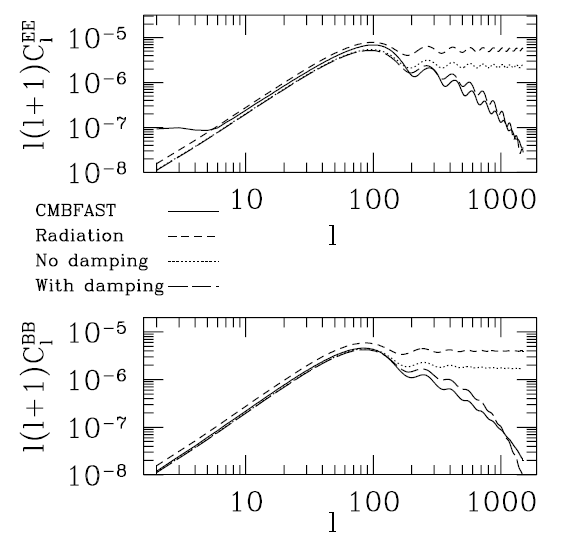
\includegraphics[width=0.5\linewidth]{analytic.png}
  \centering
  \label{analytic1}
  \caption{Comparison of E and B power spectra from CMBFAST (solid curve) with (semi)analytic approximations. The (semi)analytic solutions use forms for h in radiation domination, calculated numerically, and calculated numerically  with exponential damping}
\end{figure}


Throughout we have taken the visibility function to be near Gaussian, and peaked around polarisation. We know however CMB photons scatter further at reionisation, which modifies the above discussion. Similarly to recombination, this contributes a peak at a new scale, that of the horizon size at $\tau_{re}$, to the polarisation power sepctra. Since the horizon is growing, this peak is at a larger angular scale contribution than the recombination peak, at roughly $l<10$. It also contributes a further exponential suppression at small scales \cite{reionisation2}.\\

Through carefully going through an analytic understanding of these power spectra, we have uncovered certain parameters and scales that can be probed provided a sufficiently precise measurement of the B mode spectrum. Tensor power spectra are sensitive to three main scales: the horizon scale at recombination, the horizon scale at matter-radiation equality, and the width of the SLS, among other cosmological parameters. In the near future we don't expect to be able to measure this full spectrum, and so for the purposes of this essay and for an initial measurement of $r$, the existence of the power spectrum peak at fixed known $l$ and predictable size given $r$ is the key result.



\subsection{Scalar Perturbations}

For completeness we should discuss scalar perturbations too. Importantly, these do not produce a B mode polarisation, a fact for which we give just some intuition for here, though one can perform an entirely analogous analysis for scalars also. As before, we work in Fourier space with wave vector $\v{k}$, which we may choose to be aligned with the $\unit{z}$ direction, and take the basis on which we evaluate $Q$ and $U$ to be the natural basis on the sphere: $(\unit{e}_1, \unit{e}_2) = (\unit{e}_\theta, \unit{e}_\phi)$. The angular dependence of this system, and therefore of the Boltzmann equations too, turn out this time to only be in the dot product of relevant directions $\mu=\v{k}\cdot\unit{n}$, unlike for tensor perturbations which also have azimuthal dependence. The scalar quadrupole moment generated therefore has no $\phi$ dependence, i.e. is the $m=0$ mode, and so generates azimuthally symmetric polarisation. Thus, recalling Q describes the difference in power between the $\unit{e}_\theta$ and $\unit{e}_\phi$ directions, we see Q is non zero as polarisation is aligned with $\unit{e}_\theta$. U on the other hand is not, as it measures the difference of power between $\unit{e}_\theta\pm\unit{e}_\phi$, which are equal. Another way to say the same thing is that the polarisation eigenvector must be proportional to $\unit{e}_\theta$, which by the form of the polarisation matrix forces $U=0$. Now by \ref{EBmodes}, we see if $U=0$, then $B(\unit{n})$ is identically 0. One can think of the additional linearly independent degree of freedom in tensor perturbations being responsible for their azimuthal dependence, which results in both Q and U and so both E and B mode polarisation being generated. 


\newpage
\section{Observing B modes}


We have seen that primordial perturbations induce characteristic polarisation signals in the CMB. The significance of the E/B decomposition is now clear, since

\begin{enumerate}
\item Scalar (density) perturbations create only E modes, and no B modes
\item Vector (vorticity) perturbations create mainly B modes
\item Tensor (gravitational wave) perturbations create both E and B modes
\end{enumerate}

In the previous section we showed (1) and (3). We omitted showing (2) since it can be shown that vector perturbations redshift away rapidly due to cosmic expansion, and so are not expected to contribute significantly to the observed B-mode signal  \cite{vector}. The fact that scalars do not produce B-modes while tensors do is the basis for the claim that a detection of B-modes is `smoking-gun'  evidence for inflation \cite{smokinggun}. The search for these B-modes is thus a major focus of observational cosmology - a detection will have far reaching consequences for the entire theoretical physics community. \\

Having motivated the search for B-modes, we now turn to a number of issues in their detection. To be sure we have detected primordial gravitational waves, we must be sure a measured signal can only be attributed to them, not generated by some other effect. We discuss three points here, in varying levels of detail. Firstly, other possible sources of B modes in the early universe. Secondly, the issue of foregrounds: emission from other sources obscuring the CMB polarisation signal. Finally, and most interestingly, the weak gravitational lensing of CMB photons by intervening matter between us and the surface of last scattering. These issues, combined with the fact that the expected amplitude of B mode signal is tiny, makes their detection a daunting task.


\subsection{Other Primordial B modes}
\label{vectorissues}

A number of other early universe effects are capable of producing B modes after the epoch of inflation, and our analysis should account for the possibility that these contribute too. We use the illustrative example of topological defects which may generate observable B modes even in the absence of IGWs. These are generically found in supersymettric grand unification models \cite{CMBPol}.\\

The best studied phenomena is that of cosmic strings, formed at the end of multi-field inflation upon the breaking of a $U(1)$ symmetry. If formed, they would induce a B-mode polarisation in the CMB through continously sourced vector perturbations after inflation, which are no longer negligible as they havn't redshifted away at recombination or reionisation. They predict a spectrum with two peaks, at $l\approx10$ from reionisation and $l\approx 600-1000$ from last-scattering. Recent work has found that topological defects alone cannot explain the measured BICEP-2 B-mode signal, though may be present in combination with tensor or dust contributions \cite{baddefects}.\\

Other primordial B modes may be generated by phase transitions \cite{phase} or primordial magnetic fields \cite{magnetic}, each with their own characteristic spectra.

\subsection{Foregrounds}

Unfortunately, spread out between us and the last-scattering surface at $z\approx 1100$, there is a long line of obtruding foregrounds that hinder our ability to accurately measure the CMB fields. In this brief section we give an overview of the main astrophysical or atmospheric foregrounds that contaminate our CMB polarisation signal, and describe how we may go about dealing with them. We draw from \cite{thesis} and \cite{foregrounds}.\\

Recall first that the CMB is a near perfect black body emitter, with a characteristic frequency profile given by the Planck distribution peaking at about 160Ghz. Foregrounds can broadly be seperated into three classes: atmospheric, galactic, or extragalactic. Each individual type of foreground has its own distinctive frequency dependence, and degree of polarisation. Those contributing at CMB frequencies are summarised in figure \ref{foregrounds}. We see the main contaminants for our studies of polarisation are galactic in origin, from synchrotron emission at low frequencies below 100Ghz, and thermal dust at higher frequencies. The other contaminants listed in the top panel turn out to not be significantly polarised so don't pose too much of an issue. The bottom panel further shows this really is a large problem! The expected B mode signal, even for a relatively large value of $r\approx0.1$ falls below the average polarised foreground level on the full sky at all CMB frequencies.\\

\begin{figure}[h]
  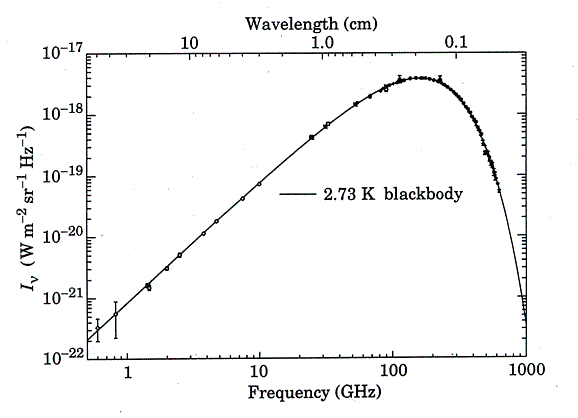
\includegraphics[width=0.4\linewidth]{cmbspectrum1.png}
  \centering
  \caption{the CMB spectrum as measured by the COBE sattelite, matches that of a black body emitter at the CMB temperature - image from https://webhome.phy.duke.edu/~kolena/cmb.html  }
\end{figure}

\begin{figure}[h]
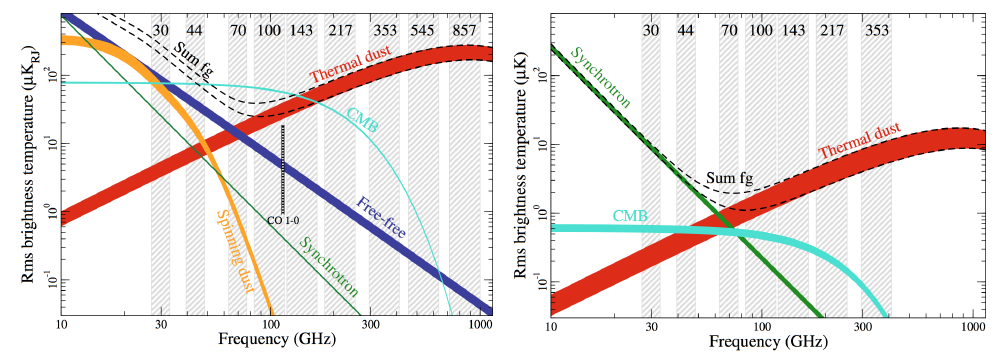
\includegraphics[width=0.4\linewidth]{foregrounds.png}
\centering
\caption{Spectral energy distributions (SED) of relevant astrophysical foregrounds. The top panel are the main contributions to temperature, and the bottom, for polarisation. The shaded bars indicate the observation frequencies for the Planck satellite, and the upper and lower limits correspond to masks with different sky fractions used (81 and 93\%). Image from \cite{planck2016b}.}
\label{foregrounds}
\end{figure}

\textbf{Atomospheric effects}: Absorption lines from oxygen at 60 and 120 Ghz, and water vapour at 20 and 18Ghz limit access to the microwave sky. Thermal emission from the atmosphere is unpolarised, though Zeeman splitting of oxygen lines in Earth's magnetic field leads to polarized emission, which is primarily circularly polarized. While the CMB is not expected to be circularly polarized, instrumental issues could lead to a $\approx 0.01\%$ circular-to-linear polarisation conversion, which could still lead to a measured B mode signal orders of magnitude larger than if $r=0.01$, say. Backscattering of thermal radiation emitted by the earths surface off ice  crystal clouds in the troposphere may also give B mode signals larger than the expected CMB B mode signal. \\

\textbf{Galactic Synchrotron emission}: This emission is produced by acceleration of charged particles in interstellar magnetic fields. Via multi frequency measurements from the WMAP and Planck sattelites, we find a very good fit to SED $T_d(\nu) \propto \nu^{\beta_s}$ with $\beta_s \approx -3$, which varies slightly over the sky, due to the dependence on the acceleration of charged particles.\\

\textbf{Galactic Dust}: This emission is produced due to presence of dust grains in the interstellar medium. In dense regions of star formation, UV radiation from newly formed stars heats up nearby dust, which radiate strongly polarised light in the IR and microwave frequencies. The grain size and dust temperature determine the spectral properties of the radiation, which can be fitted well to a modified black body emission spectrum $T_d(\nu) \propto \nu ^ {\beta_d+1}[e^{\nu/T}-1]^{-1}$. Measurements from Planck show $T_d$ and spectral parameter $\beta_d$ vary over the sky, with average values differing significantly in and out of the galactic plane. While no region of the sky was found to be sufficiently clean of dust to require no foreground removal for clean B mode measurements, Planck did identify certain patches of the sky with considerably lower foreground amplitudes, which may be of use in future CMB missions. \\

The statistical algorithms and methods designed to separate these foregrounds from the clean CMB (the primary signal plus secondary effects) are known as CMB component separation \cite{componentsep}, and make use of several datasets. They can be grouped into two classes. Non blind methods attempt to make use of the known spectral frequency properties of certain foregrounds, while blind assume little or no prior information about the form of the foregrounds, instead relying on their statistics: different foregrounds should be statistically independent, and the statistics of the primary CMB are well understood from theory.\\

Proper foreground removal is very important. In order to detect a primordial B mode signal at $r=0.01$ at a $3\sigma$ significance for example, we must only have a $1\%$ level of residual foregrounds. It is however easy to go wrong. In March 2014 the BICEP2 Collaboration reported detection of B-mode power at 150 GHz in the range $40<l<100$, in excess of that expected from lensing (see next section), and greater than that expected from foregrounds \cite{bicep2cockup}. This would have been huge \cite{smokinggun}, however unfortunately, under further scrutiny, arguments were made that uncertainties in the various dust templates may have been underestimated. By cross correlating with newer BICEP2/Keck and Planck it was found that this entire excess B mode could be attributed to dust, leaving again only an upper bound on $r$ \cite{bicep2cockup2}.


\subsection{CMB Lensing}
\label{lensing}
CMB lensing is the deflection of CMB photons by all intervening matter in the universe by gravity. It is a second order effect and is thus not treated in the linearised boltzmann equation formalism used to describe the CMB so far. While in the linear regime each Fourier mode evolves independently, lensing mixing these Fourier modes, making the statistics of the lensed sky far more complicated than those of the unlensed one. \\

We treat lensing in the `weak lensing' regime, where images (and also generally other fields on the sphere) experience a small shift compared to the original unlensed field. The effect of gravitational lensing is greatest when the lens (i.e. the matter responsible for the deflection) is massive, and close to the source. While some lenses for the CMB are certainly massive, they are relatively far from the $z\approx1100$ source, since structure doesn't form in the universe until a much later time. The opposing `strong lensing' regime is also very interesting, though not relevant here.\\

Lensing affects all three of our observable CMB fields: the temperature fluctuation $T$, and Stokes parameters $Q$ and $U$, and in doing so also the derived physical $E$ and $B$ fields in a way that will be made precise later. It has the effect of locally (i.e. on small patches of the sky) sqaushing and stretching the CMB, shifting local power spectra towards lower or higher angular scales. Summing over many patches we see a small smoothing of oscillations in the temperature and E mode spectra at a measurable several percent, rendering the effect important in precision cosmology. \\

Importantly, it also has the effect of converting some primordial E modes into lensed B modes, which we demonstrate and quantify in the flat sky limit. This obscures the primordial B mode signal, and so lensing acts as a nuisance for our studies of the primary CMB.  A typical analysis of the CMB assumes Gaussianity and statistical isotropy, giving us just a power spectrum. Lensing however introduces small amounts of non-Gaussianity, and statistical anisotropy into the CMB, so can be thought of as adding information which may be used to probe the matter distribution of the universe at out to further redshifts than possible with current galaxy surveys \cite{sloan}.

\subsubsection{Mathematical Description of Lensing}

The mathematical formalism used to describe lensing for our purposes is rather simple, and described in great detail in \cite{lewis}, on which much of this section is based. From general relativity and a flat\footnote{similar expressions exist in positive and negative curvature universes} FLRW metric, one can derive an expression for the displacement vector $\v{\alpha}$ on the sphere, dependent on observed direction $\unit{n}$, by which the lensed and unlensed fields differ. 

\begin{equation}
\tilde{X}(\unit{n}) = X(\unit{n}+\v{\alpha})
\end{equation}

\begin{equation}
\v{\alpha} = -2 \int_0^{\chi_*}d\chi \frac{\chi_*-\chi}{\chi_*\chi}\nabla_{\unit{n}}\Psi(\chi\unit{n},\tau_0-\chi)
\end{equation}

Throughout this section a tilde indicates a lensed field, not to be confused with how we defined $\tilde{E}$ and $\tilde{B}$ previously. $X$ is an observable field: $X \in \{ T, U, V\}$, $\chi$ is conformal distance, $\tau_0-\chi$ is the conformal time at which the photon was at position $\chi\unit{n}$, $\nabla_{\unit{n}}$ is the angular derivative, or equivalently covariant derivative on the sphere, and $\Psi=\half(\Psi_N+\Phi_N)$ is the Weyl potential, written in terms of the Newtonian potentials \ref{metricperturb}. We have used here the Born approximation - the line of sight integral is performed along the unperturbed geodesic path, valid as we work to first order in $\Psi$, which has been shown to be a very good approximation. $\Psi$ is related to matter perturbations by the Poisson Equation
\begin{equation}
\nabla^2\Psi = 4\pi G\bar{\delta\rho}
\label{poisson}
\end{equation}

where $\bar{\delta\rho}$ is the comoving total density perturbation, i.e. evaluated in its rest frame, and we have assumed no anisotropic stress. It is convenient to write the deflection angle instead in terms of a lensing potential
\begin{equation}\begin{split}
\psi(\unit{n}) &= -2 \int_0^{\chi_*}d\chi \frac{\chi_*-\chi}{\chi_*\chi}\Psi(\chi\unit{n},\tau_0-\chi)\\
\v{\alpha} &= \nabla \psi
\end{split}\end{equation}

One may worry about the lensing potential being divergent as $\chi \rightarrow 0$. We can amend this by setting the monopole of $\psi$ to 0, which doesn't modify $\v{\alpha}$. 

\subsubsection{Lensing Potential Power Spectrum}

We ultimately wish to calculate the lensed power spectra in terms of the unlensed. In doing so, we will need the lensing potential power spectrum. Here we derive an expression for it, showing it is simply a weighted matter power spectrum. We make use of Fourier space the expression
\begin{equation}
\langle \Psi(\v{k},\tau,\tau')\Psi^*(\v{k}',\tau,\tau')\rangle=\frac{2\pi}{k^3}\Delta^2_\Psi(k,\tau,\tau')(2\pi)^3\delta(\v{k}-\v{k}')
\end{equation}

to get 
\begin{equation}\begin{split}
\langle \psi(\unit{n})\psi(\unit{n}') \rangle &= 4\int d\chi \int d\chi'(\frac{\chi_*-\chi}{\chi_*\chi})(\frac{\chi_*-\chi'}{\chi_*\chi'})\fint{k}\frac{2\pi^2}{k^3}\Delta^2_\Psi(k,\tau,\tau')e^{i\v{k}\cdot\v{x}}e^{-i\v{k}\cdot\v{x'}}\\
&= 16\pi \sum_{ll'mm'}\int d\chi \int d\chi'(\frac{\chi_*-\chi}{\chi_*\chi})(\frac{\chi_*-\chi'}{\chi_*\chi'})\int \frac{dk}{k}j_l(k\chi)j_{l'}(k\chi')Y_{lm}(\unit{n})Y^*_{l'm'}(\unit{n}')\delta_{ll'}\delta_{mm'}
\end{split}\end{equation}

where we have made use of the Rayleigh Plane Wave identity with $\v{x}=\chi\unit{n}$
\begin{equation}
e^{i\v{k}\cdot\v{x}} = 4\pi\sum_{lm}i^lj_l(k\chi)Y_{lm}^*(\unit{n})Y_{lm}(\unit{k})
\end{equation}

and performed the angular $\unit{k}$ using orthogonality of spherical harmonics. Finally we expand
\begin{equation}
\psi(\unit{n}) = \sum_{lm}\psi_{lm}Y_{lm}(\unit{n})
\end{equation}

and recalling the definition of $C_l^{\psi\psi}$
\begin{equation}
\langle \psi_{lm}\psi_{l'm'}^* \rangle = \delta_{ll'}\delta_{mm'}C_l^{\psi\psi}
\end{equation}

read off the angular power spectrum
\begin{equation}
C_l^{\psi\psi} = 16\pi \int_0^{\chi_*} d\chi \int_0^{\chi_*} d\chi' \int \frac{dk}{k} (\frac{\chi_*-\chi}{\chi_*\chi})(\frac{\chi_*-\chi'}{\chi_*\chi'})j_l(k\chi)j_l(k\chi')\Delta^2_\Psi(k, \tau_0-\chi, \tau_0-\chi')
\end{equation}

To make the relation with scalar perturbations explicit, we may relate this to primordial perturbations via a transfer function $\Psi(\v{k},\tau)=T_\Psi(k,\tau)\zeta(\v{k})$, giving
\begin{equation}
C_l^{\psi\psi} = 16\pi \int \frac{dk}{k} P_s(k) \left[\int_0^{\chi_*} d\chi j_l(\chi) (\frac{\chi_*-\chi}{\chi_*\chi})T_\Psi(k, \tau_0-\chi)\right]^2
\end{equation}

Alternatively, we may relate the scale invariant power spectrum of $\Psi$ to the matter power spectrum via Fourier transforming the Poisson Equation \ref{poisson}, making concrete the claim the lensing potential power spectrum is a weighted matter power spectrum.
\begin{equation}
\Delta^2_\Psi(k,\tau) = \frac{9\Omega^2_mH^4(\tau)}{8\pi^2}\frac{P_m(k,\tau)}{k}
\end{equation}

\subsubsection{Lensing of B modes} 

In this section we calculate, in the flat sky regime, the effect lensing has on temperature, E mode, and importantly, B mode power spectra. We start with temperature, and will see the polarisation calculations following similarly. We use here the series expansion approach, which gives good intuition and qualitatively correct results, though is not a good approximation on all scales. A more accurate approach instead works with real space correlation functions directly. Expanding,
\begin{equation}
\tilde{T}(\unit{n}) = T(\unit{n}+\nabla\psi) =T(\unit{n})+\nabla^a\psi(\unit{n})\nabla_aT(\unit{n})+\half\nabla^a\psi(\unit{n})\nabla^b\psi(\unit{n})\nabla_a\nabla_bT(\unit{n})+O(\psi^3)
\end{equation}

Fourier transforming and using the convolution theorem we obtain
\begin{equation}\begin{split}
\tilde{T}(\v{l}) &= T(\v{l}) - \finttwo{l_1} \v{l_1}\cdot(\v{l}-\v{l_1})T(\v{l_1})\psi(\v{l}-\v{l_1}) \\
& \qquad \quad -\half \finttwo{l_1}\finttwo{l_2}\v{l_1}\cdot(\v{l_1}+\v{l_2}-\v{l})\v{l_1}\cdot\v{l_2}T(\v{l_1})\psi(\v{l_2})\psi^*(\v{l_1}+\v{l_2}-\v{l})\\
&= T(\v{l}) - \finttwo{l_1} T(\v{l_1})L(\v{l},\v{l_1})
\label{lensedtemp}
\end{split}\end{equation}

making use of $\psi(\v{l})=\psi^*(-\v{l})$, and where we have defined 
\begin{equation}
L(\v{l},\v{l_1}) = \v{l_1}\cdot(\v{l}-\v{l_1})\psi(\v{l}-\v{l_1})+\finttwo{l_2}\v{l_1}\cdot(\v{l_1}+\v{l_2}-\v{l})\v{l_1}\cdot\v{l_2}\psi(\v{l_2})\psi^*(\v{l_1}+\v{l_2}-\v{l})\\
\end{equation}

Now in the flat sky limit the appropriate definition of  the (lensed) power spectrum is
\begin{equation}
\langle T^*(\v{l})T(\v{l}')\rangle = (2\pi)^2\delta(\v{l}-\v{l}')C_l^{TT}
\end{equation}

To lowest order in the lensing potential power spectrum, we calculate, using the fact that $T$ and $\psi$ don't correlate, and Wick's theorem
\begin{equation}\begin{split}
\tilde{C}_l^{T T} &\approx C_l^{T T}+\finttwo{l_1}[ \v{l_1}\cdot(\v{l}-\v{l_1})]^2 C^\psi_{|\v{l}-\v{l_1}|}C_{l_1}^{TT} - C_l^{TT}\finttwo{l_1} [\v{l}\cdot\v{l_1}]^2C_{l_1}^{\psi\psi}\\
&=(1-l^2R^\psi)C_l^{TT}+\finttwo{l_1}[ \v{l_1}\cdot(\v{l}-\v{l_1})]^2 C^{\psi}_{|\v{l}-\v{l_1}|}C_{l_1}^{TT}
\end{split}\end{equation}

where we have defined
\begin{equation}
R^\psi = \frac{1}{4\pi}\int \frac{dl}{l} l^4 C_l^{\psi\psi}
\end{equation}

For polarisation, the calculation is rather similar. Recall that in the flat sky limit we must rotate Q and U Fourier modes into E and B modes as \ref{QUrotateflat}
\begin{equation}\begin{split}
 P_{\pm} (\unit{n}) := (Q\pm iU)(\unit{n})  &= \finttwo{l}(E(\v{l})\pm i B(\v{l}))e^{\pm 2i\phi_{\v{l}}}e^{i\v{l}\cdot\unit{n}}\\
\Leftrightarrow  P_{\pm}(\v{l}) &= (E(\v{l})\pm i B(\v{l}))e^{\pm 2i\phi_{\v{l}}}
\label{relationship}
\end{split}\end{equation}

Now lensing acts on $P_{\pm}$ exactly as it did on the temperature field 
\begin{equation}
\tilde{P}_{\pm}(\unit{n}) = P_{\pm}(\unit{n}+\nabla\psi) =P_{\pm}(\unit{n})+\nabla^a\psi(\unit{n})\nabla_aP_{\pm}(\unit{n})+\half\nabla^a\psi(\unit{n})\nabla^b\psi(\unit{n})\nabla_a\nabla_bP_{\pm}(\unit{n})
\end{equation}

which in Fourier space gives
\begin{equation}
\tilde{P}_{\pm}(\v{l}) \approx P_{\pm}(\v{l}) - \finttwo{l_1} P_{\pm}(\v{l_1})L(\v{l},\v{l_1})
\end{equation}

Finally to we use the relationship \ref{relationship} between $P_\pm$ and $E$ and $B$ modes twice
\begin{equation}\begin{split}
\tilde{E}(\v{l})\pm i\tilde{B}(\v{l}) &= e^{\mp 2i\phi_\v{l}}\tilde{P}_{\pm}(\v{l})\\
&=e^{\mp 2i\phi_\v{l}}\left(P_{\pm}(\v{l}) - \finttwo{l_1} P_{\pm}(\v{l_1})L(\v{l},\v{l_1})\right)\\
&=E(\v{l})\pm iB(\v{l})-\finttwo{l_1} e^{\pm 2i(\phi_\v{l_1}-\phi_\v{l})}(E(\v{l_1})\pm iB(\v{l_1}))L(\v{l},\v{l_1})
\label{lensedEBmodes}
\end{split}\end{equation}

%&=e^{\mp 2i\phi_\v{l}}(e^{\pm 2i\phi_\v{l}}(E(\v{l})\pm iB(\v{l}))-\finttwo{l_1} e^{+2i\phi_\v{l_1}}(E(\v{l_1})\pm iB(\v{l_1}))L(\v{l},\v{l_1}))\\


departing from the temperature case in this phase factor. Now we may calculate lensed power spectra involving polarisation fields
\begin{equation}
\langle E^*(\v{l})E(\v{l}')\rangle = (2\pi)^2\delta(\v{l}-\v{l}')C_l^{EE} \qquad \langle B^*(\v{l})B(\v{l}')\rangle = (2\pi)^2\delta(\v{l}-\v{l}')C_l^{BB}
\end{equation}

and also $C_l^{TE}$ omitted. Schematically, this calculation is similar to that for lensed temperature perturbations, and we pick up identical terms. By correlating $\tilde{E}(\v{l})\pm i\tilde{B}(\v{l})$ with itself and $\tilde{E}(\v{l})\mp i\tilde{B}(\v{l})$ we obtain

\begin{equation}\begin{split}
\tilde{C}_l^{EE}+\tilde{C}_l^{BB} \approx C_l^{EE}+C_l^{BB}&+\finttwo{l_1}[ \v{l_1}\cdot(\v{l}-\v{l_1})]^2 C^\psi_{|\v{l}-\v{l_1}|}(C_{l_1}^{EE}+C_{l_1}^{BB}) \\
&- (C_{l}^{EE}+C_{l}^{BB})\finttwo{l_1} [\v{l}\cdot\v{l_1}]^2C_{l_1}^{\psi\psi}\\
\tilde{C}_l^{EE}-\tilde{C}_l^{BB} \approx C_l^{EE}-C_l^{BB}&+\finttwo{l_1}e^{4i(\phi_{\v{l_1}}-\phi_\v{l})}[ \v{l_1}\cdot(\v{l}-\v{l_1})]^2 C^\psi_{|\v{l}-\v{l_1}|}(C_{l_1}^{EE}-C_{l_1}^{BB})\\
&- (C_{l}^{EE}-C_{l}^{BB})\finttwo{l_1} )[\v{l}\cdot\v{l_1}]^2C_{l_1}^{\psi\psi}
\end{split}\end{equation}

The integrals are actually all real by symmetry in $\v{l_1}$, and so we may replace the exponentials by cosines. Adding and subtracting we get

\begin{equation}\begin{split}
\tilde{C}_l^{EE} &= (1-l^2R^\psi)C_l^{EE}+\half \finttwo{l_1}[ \v{l_1}\cdot(\v{l}-\v{l_1})]^2 C^\psi_{|\v{l}-\v{l_1}|}\\
&\qquad \times [(C_{l_1}^{EE}+C_{l_1}^{BB})+\cos{4(\phi_\v{l_1}-\phi_\v{l})}(C_{l_1}^{EE}+C_{l_1}^{BB})]\\
\tilde{C}_l^{BB} &= (1-l^2R^\psi)C_l^{BB}+\half \finttwo{l_1}[ \v{l_1}\cdot(\v{l}-\v{l_1})]^2 C^\psi_{|\v{l}-\v{l_1}|}\\
&\qquad \times [(C_{l_1}^{EE}+C_{l_1}^{BB})-\cos{4(\phi_\v{l_1}-\phi_\v{l})}(C_{l_1}^{EE}+C_{l_1}^{BB})]\\
\label{lensedBmodes}
\end{split}\end{equation}

Here comes the key point: even if $C_{l}^{BB}$ is zero, i.e. the unlensed field has no B modes sourced by primordial inflationary gravitational waves, lensing creates some. This has important consequences for the detectability of B modes from gravitational modes.\\

We saw tensor modes generate their largest signal on large angular scales $l<100$ so we seek to understand lensing B modes in that range. Taking $C_l^{BB}=0$ we find for $|\v{l}| \ll |\v{l_1}|$ that 

\begin{equation}\begin{split}
\tilde{C}_l^{BB} &= \half \finttwo{l_1}[ \v{l_1}\cdot(\v{l}-\v{l_1})]^2 C^\psi_{|\v{l}-\v{l_1}|}C_{l_1}^{EE}\sin^2{2(\phi_\v{l_1}-\phi_\v{l})}\\
&\approx \finttwo{l_1} l_1^4C^{\psi\psi}_{l_1}C^{EE}_{l_1}\sin^2{2(\phi_\v{l_1}-\phi_\v{l})}\\
&=\frac{1}{4\pi}\int \frac{dl_1}{l_1}l_1^6C^{\psi\psi}_{l_1}C^{EE}_{l_1}
\end{split}\end{equation}

independent of l. This corresponds to a white noise spectrum independent of l for small l, a very good approximation for roughly $l\ll 1000$, the range over which we would want to observe B modes. The power spectra of $\psi$ is related to the matter power spectrum and is well understood. The power spectrum of unlensed $E$ is approximately the measured lensed $E$, and can also be predicted from theory assuming it is sourced primarily from scalar perturbations. These suffice to give a good approximation for the size of this white noise effect: $\tilde{C}_l^{BB} \approx 2\times10^{-6}\mu K^2$, corresponding to an instrumental white-noise level of $\approx 5\mu$K-arcmin.\\

\begin{figure}[h]
  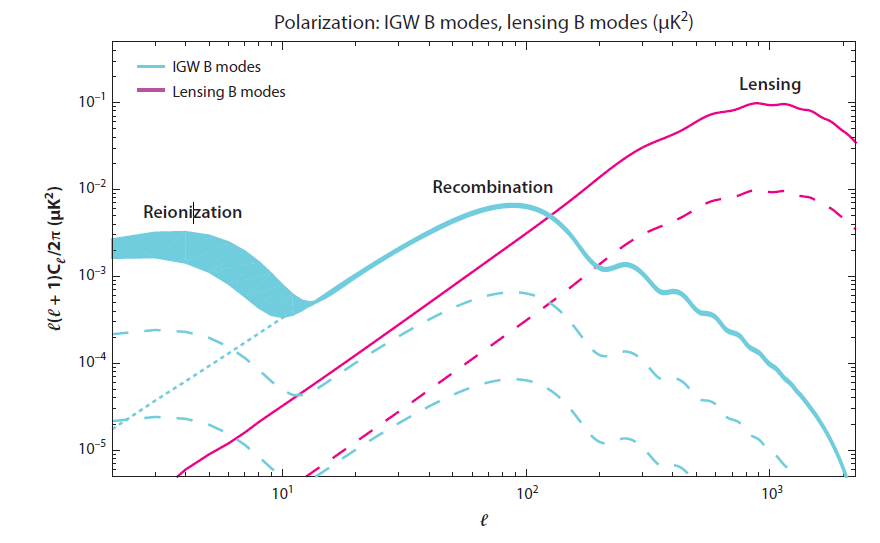
\includegraphics[width=0.7\linewidth]{lensingfucksus.png}
  \centering
  \caption{Polarisation power. Spectra are shown for primordial B modes with $r=\{0.1,0.01,0.001\}$ in cyan, and lensing induced B modes in magenta. The $\pm1\sigma$ uncertainity is due to the current constraint on $\kappa$, the optical depth to reionization and shown for $r=0.1$. The cyan dotted line is the result with no reionization. a 90\% delensed signal is shown in dotted magenta. Plots generated using CAMB \cite{CAMBInfo}, and taken from \cite{QBM}}
  \label{lensingisfucked}
\end{figure}

We are now in a position to demonstrate how large a problem lensing is. Figure \ref{lensingisfucked} plots the power spectrum of primordial B modes from IGWs for various values of $r$. It also plots the power of lensed B modes over the region we expect to see an inflationary B mode signal. We see the lensing contribution obscures IGW B modes, though for r sufficiently large: i.e. within roughly an order of magnitude of the current upper bound, the recombination peak may may still stand out. Several experiments have confirmed detection of these lensing B modes in the range $200<l<1500$, for example first in 2014 by the POLARBEAR collaboration \cite{polarbear}. Shown also on the figure is an ambitious delensed signal, which we discuss next.

\subsubsection{Delensing}

In the limit of small instrumental noise, the dominant source of B-mode power on large angular scales is gravitational lensing. For instrumental noise levels falling below the lensing white noise experiments will be lensing-limited: the limiting factor in constraining r will be the lensing B-mode. While foregrounds can be removed through exploiting multifrequency data, this is not possible for lensing. Instead, delensing algorithms have been proposed  which statistically separate the gravitational wave and lensing B-mode signals, offering the prospect for reducing the noise floor and unlocking more modes for observation. These algorithms are based on a relatively simple idea: given information about noisy observed E modes, together with information about the lensing potential and therefore the deflection field, we can estimate the large-scale lensing B-mode and subtract it from the observed B-mode.\\

The required estimate for the defection field can be any probe of the universes matter distribution -  it may be obtained externally or internally. A promising external probe is the cosmic IR background, emitted by UV heated dust surrounding early stars, due to its high degree of correlation with the lensing signal \cite{sherwin}. Typically however an internal estimate is used, i.e. from the CMB itself, and we give an example of one such estimator in the next section. \\

Given an such an estimator $\hat{\psi}(\v{l})$, we may use the lensed E mode as a proxy for the unlensed E mode, and write, via taking the imaginary part of \ref{lensedEBmodes}
\begin{equation}
B^{\text{reconstructed}}(\v{l}) = \finttwo{l_1} \v{l_1}\cdot(\v{l}-\v{l_1}) \tilde{E}(\v{l_1})\hat{\psi}(\v{l}-\v{l_1})\sin[2(\phi_\v{l_1}-\phi_\v{l})]
\label{sin}
\end{equation} 

which we then subtract off of our observed B modes, getting a delensed mode
\begin{equation}
B^{\text{delensed}}(\v{l}) = B^{\text{observed}}(\v{l}) - B^{\text{reconstructed}}(\v{l})
\end{equation}

The degree to which the B mode signal can be delensed ultimately depends on how well this reconstruction of $\psi$ can be accomplished. 

\subsubsection{Lensing Reconstruction}

The step we brushed under the rug above was the reconstruction of the lensing potential. Here we discuss the simplest of such estimators as in \cite{hu-estimator,lewis}, which have recently been used to create lensing mass maps over large portions of the sky by the ACT collaboration \cite{darwish}. \\

The idea here is that the unlensed CMB is statistically very simple - it is Gaussian, i.e. distinct Fourier modes are statistically independent: $\langle X^*(\v{l})X(\v{l'})\rangle =0$ for  $\v{l} \neq \v{l'}$. Lensing, being a non linear effect mixes these Fourier modes: we saw above by the convolution theorem that  $\tilde{X}(\v{l})$ picks up contributions from all modes ${X}(\v{l_1})$ and $\phi(\v{l_2})$ with $\v{l_1}+\v{l_2}=\v{l}$. It thus contains information about the lensing potential.\\

Let us demonstrate this explicitly for the case of temperature perturbations. From the expression \ref{lensedtemp} we calculate the average over many CMB
%got rid of _T
\begin{equation}\begin{split}
\langle \tilde{T}(\v{l})\tilde{T}^*(\v{l}-\v{L})\rangle &= \delta(\v{L})C_l^{TT} \finttwo{l_1}  \v{l_1}\cdot(\v{l}-\v{l_1})\psi(\v{l}-\v{l_1}) \langle T(\v{l_1})T^*(\v{l}-\v{L})\rangle + O(\psi^2) \\
&\qquad + \v{l_1}\cdot(\v{l}-\v{L}-\v{l_1})\psi^*(\v{l}-\v{L}-\v{l_1}) \langle T(\v{l})T^*(\v{l_1})\rangle\\
&=\delta(\v{L})C_l^{TT} + [(\v{L}-\v{l})\cdot\v{L}C^{TT}_{|\v{l}-\v{L}|}+\v{l}\cdot\v{L}C_l^{TT}]\psi(\v{l}) + O(\psi^2)
\end{split}\end{equation}

The $\v{L}\neq 0 $ modes therefore probe the lensing potential. To estimate the lensing potential we perform a weighted average of all off diagonal terms
\begin{equation}
\hat{\psi}(\v{L}) = N(\v{L})\finttwo{l} \tilde{T}(\v{l})\tilde{T}^*(\v{l-L})g(\v{l},\v{L})
\end{equation}

where $g(\v{l},\v{L})$ is some weighting function. To be unbiased at lowest order we want the estimator to be unbiased $\langle \hat{\psi}(\v{L}) \rangle = \psi(\v{L})$, which by the previous calculation gives
\begin{equation}
N(\v{L})^{-1} = \finttwo{l} [(\v{L}-\v{l})\cdot\v{L}C^{TT}_{|\v{l}-\v{L}|}+\v{l}\cdot\v{L}C_l^{TT}]g(\v{l},\v{L})
\end{equation}

We now choose $g$ to maximise the signal to noise. One can compute the variance to zeroth order in $C_l^{\psi\psi}$ as $\langle| \hat{\psi}(\v{L})-\psi(\v{L})|^2 \rangle \approx 
\langle| \hat{\psi}(\v{L})|^2 \rangle$ as

\begin{equation}
\langle\hat{\psi}^*(\v{L}) \hat{\psi}(\v{L}) \rangle = \delta(\v{0})2N(\v{L})^2\finttwo{l}\tilde{C}_l^{tot}\tilde{C}_{|\v{l}-\v{L}|}^{tot}g(\v{l},\v{L})^2 + O(C_l^{\psi\psi})
\end{equation}

where $\tilde{C}_l^{tot} = \tilde{C}_l^{TT} + N_l$ is the total observed lensed + noise spectrum. By differentiating this variance with respect to g, we may minimize the variance to 0th order via the choice

\begin{equation}
g(\v{l},\v{L}) = \frac{[(\v{L}-\v{l})\cdot\v{L}C^{TT}_{|\v{l}-\v{L}|}+\v{l}\cdot\v{L}C_l^{TT}]}{2\tilde{C}_l^{tot}\tilde{C}_{|\v{l}-\v{L}|}^{tot}}
\end{equation}

completing the construction of the minimum variance estimator. 

\begin{equation}
\hat{\psi}(\v{L}) = N(\v{l})\v{L}\cdot\finttwo{l} \frac{C_l^{TT}\tilde{T}(\v{l})\tilde{T}(\v{L-l})}{\tilde{C}_l^{tot}\tilde{C}_{|\v{l}-\v{L}|}^{tot}}
\end{equation}


This has lowest order variance, or noise, given by


\begin{equation}
\delta(\v{0}) \langle |\hat{\psi}(\v{L})|^2 \rangle^{-1} =  N(\v{L})^{-1} = \finttwo{l}  \frac{[(\v{L}-\v{l})\cdot\v{L}C^{TT}_{|\v{l}-\v{L}|}+\v{l}\cdot\v{L}C_l^{TT}]^2}{2\tilde{C}_l^{tot}\tilde{C}_{|\v{l}-\v{L}|}^{tot}}
\end{equation}

We have constructed the estimator from solely the temperature field here. The polarisation fields also provide useful information and one can construct a total of 6 minimum variance estimators out of the three fields: $\{TT, TE, TB, EE, EB, BB\}$, each with different normalisation and weight functions, which can be found in \cite{hu-estimator}. $BB$, under the null hypothesis of $r=0$ has vanishing signal to noise so is not used. Given a sufficiently sensitive experiment the $EB$ estimator turns out to have the best signal-to-noise, and permits mapping out to $l=1000$. The reason is that that under the null hypothesis of $r=0$, the unlensed B mode has no noise, while the lensed B mode peaks at relatively high $l$, due to the presence of the sine term in \ref{sin} - see figure \ref{lensingisfucked}. This gives a large number of small-scale coherence patches in the sky in polarization, though also requires a high instrument sensitivity to exploit. If high $l$ measurements are noise limited, as is the case for Planck polarisation data, the estimators perform similarly, and can be used either together with inverse variance weighting, or to cross check each other.


\newpage
\section{Probing Inflationary Physics}
\label{probe}

The B mode diagnostic is often termed to be a `smoking gun' for inflation: if detected it would provide very strong evidence for inflation, and give us significant insight into it's physics. In this section we firstly discuss why this first statement is true, and go on to discuss what additional constraining power a detection of primordial tensors like perturbations would provide.

\subsection{Inflation Alternatives}

It is still up for debate as to whether inflation actually occurred, and a fair evaluation as to the status of inflation requires consideration of alternatives. Our confidence in inflation is twofold: firstly observational data thus far has been entirely consistent with what we might expect inflation to produce, and secondly the striking absence of compelling alternatives. While there do exist several other theories for the early universe in the literature, they all suffer serious problems. We make this concrete for the particular alternative of an \textit{Ekpyrotic} cosomology here \cite{CMBPol}.\\

One key motivation for inflation was that it necessarily causes the comoving horizon to shrink, solving the horizon problem, a problem which any contender to inflation must also deal with. Accelerated expansion is not the only mechanism that can do this: the contracting phase before a Big Crunch does so equally well. While inflation achieves shrinking $(aH)^{-1}$ via $H\approx$ const and $a(t)$ exponentially increasing, ekpyrosis relies instead on a phase of slow contraction $a(t)\approx$ const and $H^{-1}$ decreasing. This is followed by a bounce leading to the hot big bang and standard decelerating FLRW cosmology. It's cyclic extension involves our current expansion to be followed by a contracting ekpyrotic phase, leading to a new hot Big Bang phase, continuing ad infinitum.\\

It however has a major theoretical issue. For the contracting phase to smoothly connect to the expanding big bang evolution (i.e. for there to be a bounce) we require
\begin{equation}
2\Mp^2\dot{H}^2 = -(\rho + P) > 0
\end{equation} 

i.e. a violation of the null energy condition. This can be achieved at the level of an effective field theory, though so far has suffered major stability issues when attempts have been made to embed it in a UV complete theory.\\

It also has an observational issue. A simple model for the ekpyrotic cosmoology is analogous to inflation, an effective theory of a scalar field, instead rolling fast down its potential. One expects therefore the curvature perturbation to have a very blue spectrum, in stark contrast with the observed near scale invariance. Similarly the tensor spectrum is highly blue, resulting in exponentially small primordial gravitational wave amplitudes for observable modes. \\

Both points turn out to be rather representative of alternatives to inflation. Other examples include String Gas Cosmology, or Pre-Big Bang Cosmology, both rooted in String Theory. These too suffer major theoretical issues, stemming from novel and not well understood physics, which require addressing before the models can be regarded as compelling alternatives to inflation. Furthermore, they often produce negligible primordial tensor perturbations. This strengthens the constraining power of the B mode diagnostic: a detection of primordial tensor perturbations has the power to rule out some of these other models completely and really does provide strong evidence for inflation.

%\textbf{Ekpyrotic/Cyclic Cosmology}: The Ekpyrotic cosmology speculates an initial cold beginning and phase of slow contraction, followed by a bounce leading to the standard decelerating FLRW cosmology. Despite being entirely opposite to the idea of inflation, the model claims to be equally succesfull in solving the flatness and homogeneity problems.  The model has several theoretical issues: The bouncing phase requires a violation of the null energy condition, usually associated with catastrophic instabilities, and so has been hard to model consistently in a UV complete theory.\\


%\textbf{String Gas Cosmology} This postulates an initially hot dense state similar to the standard big bang cosmology. All dimensions are taken to be compact and at the string scale, with the scale inversion symettry $R\rightarrow 1/R$ fundamental to string theory. This model predicts the decompactification of three spatial dimensions, leaving the remaining dimensions stably compact, which combined with the natural hot initial state of the universe makes it appealing. The theoretical issue heres are the need for seemingly large amount of fine tuning required, as well as issues with reheating. Recent work has claimed the model is capable of generating nearly scale invariant scalar perturbations and a blue tilted spectrum of tensor perturbations, agreeing with observations thus far but distinctly different to inflation. A measurement of $n_t$ however is far in the future.\\

%\textbf{Pre-Big Bang Cosmology} Another string-theoretic model, this begins with a cold empty universe with zero curvature. Quantum fluctuations druve the universe into a scalar field driven super inflation, during which the expansion rate is increasing. This continues until the expansion rate reaches the string scale, at which point string-y corrections are required on the effective field theory description. These cause the expansion rate to be capped at a rate near the string scale, after which the universe reheats and enters radiation domination. Theoretical issues here involving the transition to radiation domination have slowed progress, and no solution to the horizon or flatness problems exist yet. This model therefore is not yet mature enough to be considered a worthy alternative to inflation




\subsection{Probes of Fundamental Physics}

Inflation so far is an excellent phenomenological paradigm for the early universe, and so it is natural to inquire about the underlying theoretical structure. In particular, how do the scalar fields involved in inflation relate to other, better understood and well tested areas of physics. A true `model of infation' is then more more than merely a choice of  effective action for some scalar fields. It it is instead an answer to at least some of the following fundamental questions \cite{CMBPol}:

\begin{enumerate}
\item Is the inflaton a particle we know about or something entirely new? 
\item How does it interact with the standard model - does it couple to the Standard Model particles through gauge interactions or in some other way? Does it couple to or involve GUT particles?
\item What is the energy scale of inflation?
\item Is inflationary physics well-approximated by semi-classical equations of motion, or are quantum effects important? 
\item Does the inflation involve extra dimensions, or a low-energy limit of string theory? 
\item How many light degrees of freedom are relevant during inflation? 
\item Is there a mechanism or symmetry principle that is responsible for the long duration of inflation?
\end{enumerate}

Theoretical physics has come a long way in mapping out a range of consistent and well-motivated inflationary mechanisms and their phenomenological predictions. However, theory alone may not distinguish between them all, and to answer these questions, some easier than others, there is a pressing need for observational data. Here we discuss the implications of a measurement of $r$, which may just be around the corner, on some of the above questions. We begin with some generic model independent results, and then discuss briefly what one can say about any particular model.\\

\textbf{Energy Scale of Inflation} \\

In the slow roll approximation, the tensor power spectrum depends only on the Hubble rate during inflation, which in SFSR models can be related to the inflaton potential via $3H^2\Mp^2\approx V$. The scalar power spectrum depends both on the Hubble rate, as well as the slow roll parameter $\epsilon$, which is directly related to the scalar to tensor ratio $r$. Given these, we may compute the energy scale of inflation. Working at the pivot scale $k_* = 0.05Mpc^{-1}$
\begin{equation}
\Delta^2_{s}\approx \frac{V}{24\pi^2\epsilon\Mp^4}
\end{equation}

Making use of $ A_s \approx 2.2\times10^{-9}$, $r\approx 16\epsilon$, and $\Mp \approx 2.43\times 10^{18} GeV$ we learn
\begin{equation}\begin{split}
V=24\pi^2A_s\frac{r}{16}\Mp^4 \Rightarrow V^{1/4} &\approx 3.22\times10^{16}\text{GeV}r_*^{1/4}\\
&= 1.04\times10^{16}\text{GeV}(\frac{r_*}{0.01})^{1/4} \\
&\leq 1.75\times10^{16}\text{GeV}
\end{split}\end{equation}

where the inequality comes from the  bound $r_*<0.1$. A detectably large tensor amplitude would be very good evidence for inflation, and demonstrate a tremendously high new fundamental energy scale in physics - comparable to that of Grand Unified Theories. Let us not understate this - this will be exceedingly important for the high energy physics community. We will have unlocked a unique probe of an energy scale roughly 12 orders of magnitude higher than possible via terrestrial collider experiments. \\

\textbf{Field Excursion}\\

As before, combining the scalar and tensor power spectrum gives information about $\epsilon$, which in the slow roll regime contains information about the background evolution of the field. In particular, recalling our previous calculation \ref{efolds} we can compute the `field excursion' of the inflaton field in planck units
\begin{equation}\begin{split}
N(t) &=  \int_{\phi(t)}^{\phi_{end}} \frac{d\phi}{\sqrt{2\epsilon}\Mp}\\
\Rightarrow dN&=\frac{d\phi}{\sqrt{2\epsilon}\Mp}\\
\Rightarrow \frac{\Delta \phi}{\Mp} &= \int_0^N \sqrt{2\epsilon} dN = \int_0^N \sqrt{\frac{r}{8}} dN 
\end{split}\end{equation}

The total field excursion between the end of inflation and the time when fluctuations were created on CMB scales is then 
\begin{equation}
\frac{\Delta \phi}{\Mp} =  \int_0^{N_*} \sqrt{\frac{r(N)}{8}} dN  = \left(\frac{r_*}{8}\right)^\half N_{\text{eff}}
\end{equation}

where $N_{eff}$ is model dependent and given by
\begin{equation}
\int_0^{N_*}\left(\frac{r(N)}{r_*}\right)^\half dN
\end{equation}

In slow roll inflation $r$ is approximately constant, but depends slightly on $N$, precisely because $\epsilon$ varies slightly during inflation. For slow roll models $r$ varies only at second order in slow roll parameters and we can estimate  $N_{\text{eff}} \approx 30-60$ to give
\begin{equation}
\frac{\Delta \phi}{\Mp} > 1.06 \times (\frac{r_*}{0.01})^{1/2}
\end{equation}

where the second inequality comes from a conservative lower limit on $N_{eff} > 30$. We see can seperate inflation models into two (vaguely) distinct classes, depending on if $r\lessapprox 0.01$ or $r\gtrapprox 0.01$, known as small and large field models. This is the Lyth bound \cite{Lyth}.\\


\begin{figure}[h]
  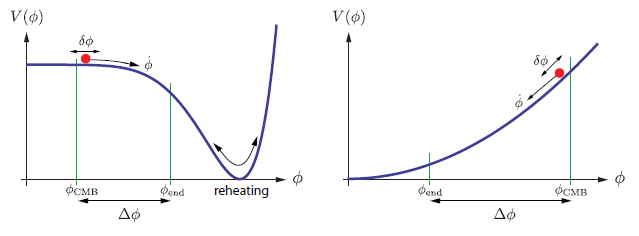
\includegraphics[width=0.7\linewidth]{smalllargefield.png}
  \centering
  \caption{Examples of typical small (left) and large (right) field models, with field excursion shown. Figure taken from \cite{baumannTASILecturesInflation2012}}
\end{figure}

While both small and large field models are challenging to construct consistently, and require some degree of fine tuning, large field models prove more difficult. Suppose we expand the inflaton potential in a SFSR model as 

\begin{equation}
V(\phi) = \half m^2\phi^2 + \sum_{p=3}^\infty \lambda_p(\frac{\phi}{\Mp})^p
\end{equation}

We can fine tune $\lambda_p$ such that at any $\phi$, $\epsilon, \eta \ll 1$, though these coefficients are expected to receive quantum corrections $\Delta\lambda_p(\phi)$, which generically will be of order unity in superplanckian field ranges, expected in large field inflation. It is hard to see inflation being maintained for sufficiently many e folds as $\epsilon, \eta << 1$ would likely not be preserved over this full range. \\

A detection (or lack thereof) of $r$ in upcoming CMB experiments, with forecasted sensitivity $r\approx 10^{-3}$, would have far reaching implications for inflationary model building. It would be able to definitively either validate or rule out such large field models, and further would give information about the full UV completion of the quantum field theory and gravity, and hence a clue towards quantum gravity.

\subsection{Inflation Models}

Having worked fairly model independently thus far, we give some examples of particular inflation models, and their general predictions for observables, focussing initially on SFSR. In this context, a model prescribes the potential $V$ and a number of e folds of inflation $N_*$ at some pivot scale, a kind of initial condition. From this, we may deduce two observational quantities of interest $n_s$ and $r$. \\

\textbf{Large field models} \\

We demonstrate the calculation alluded to above in the case of a power law potential \cite{QBM}
\begin{equation}
V(\phi) = \half m^{4-\alpha}\phi^\alpha
\end{equation}

for m a mass parameter required to give the potential the correct mass dimension. We may compute 
\begin{equation}
\epsilon_V = \frac{\Mp^2\alpha^2}{2\phi^2}
\end{equation}
	
and therefore
\begin{equation}
\begin{split}
N &= \int_{\phi_e}^\phi \frac{d\phi}{\Mp}\frac{1}{\sqrt{2\epsilon}} \\
&= \frac{1}{2\Mp^2}(\phi^2-\phi^2_e)\\
&= \frac{\alpha}{4}\left(\frac{1}{\epsilon-1}\right)
\end{split}
\end{equation}

using $\epsilon(\phi_e)=1$. This gives $\epsilon_V \approx \frac{\alpha}{4N}$ to first order in slow roll parameters. Using this, one calculates $\eta_V=\frac{\alpha-1}{2N}$. Finally we obtain
\begin{equation}
n_s-1 = -\frac{2+\alpha}{2N} \qquad r=\frac{4\alpha}{N}
\end{equation}

We may break the degeneracy by expressing  $N=N(\alpha, n_s)$, and therefore $r=r(\alpha, n_s)$, and then using the Planck best fit value of $n_s=0.968$. We can also extract the energy scale at the end of inflation as  $V(\phi_e)=m^{4-\alpha}(\frac{\alpha\Mp}{\sqrt{2}})^\alpha/2$, and also infer the field excursion.\\

Another important large field model is that of natural inflation, motivated by axions
\begin{equation}
V(\phi) \propto 1-\cos\frac{\phi}{\mu}
\end{equation}
for $\mu>\Mp$ a parameter.\\

\textbf{Small field models} \\

The hilltop model is a fairly typical looking small-field model, with

\begin{equation}
V(\phi) \propto 1-\left(\frac{\phi}{\mu}\right)^p + ... 
\end{equation}

for $p>2$, ($p=2$ turns out to be large field), and $\phi<\mu \ll \Mp$. This predicts $n_s-1 \approx \frac{-2}{N}\frac{p-1}{p-2}$ and an upper limit on $r\lesssim 8\frac{p}{N(p-2)}(\frac{8\pi}{Np(p-2)})^{p/(p-2)}$. The potential may be considered as an approximation to a generic symmetry breaking potential, with the dots denoting higher order terms becoming important near the end of inflation and during reheating. \\

These parameters provide a simple way of meeting SFSR models with observational data, as demonstrated for some of the above models and many others in figure \ref{inflationconstraints}. In general SFSR models can have a blue or red tilt, with current measurements of the primordial scalar power ruling out all blue models. From the precise shape of the data we get more stringent constraints. For progress to be made we must further constrain the range of allowed $r$ values - a detection of $r$ to any uncertainty would do so significantly, collapsing the semicircular contour in the $(n_s,r)$ plane into a tighter elliptical shape.

\begin{figure}[h]
  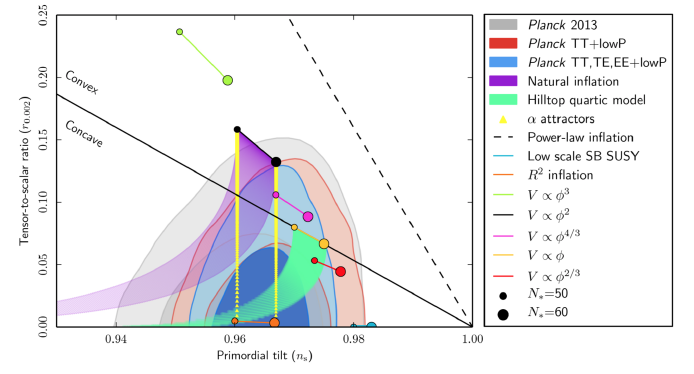
\includegraphics[width=0.7\linewidth]{modeldepconstraints.png}
  \centering
  \caption{Constraints on $n_s$ and $r$ by iterations of Planck data releases, taken from \cite{QBM}. The predictions for $N_*=50$ and $N_*=60$ from a variety of different inflationary models are shown. Concave and convex refer to the sign of the second derivative of the inflaton potential. `lowP' refers to data from the large-scale WMAP polarization survey.}
\label{inflationconstraints}  
\end{figure}


In this section we have only scratched the surface of the vast literature on inflationary models. We have worked only with SFSR models, though by taking a non trivial kinetic term in \ref{inflationaction} one gets a more generic single field model. One can also add more effective fields, extending the number of possibilities massively though diminishing predictive power, to obtain a multifield model. We can develop further plausible models by introducing a non minimal coupling to gravity, or by modifying gravity entirely, though this last one is substantially harder to do consistently \cite{baumannTASILecturesInflation2012}.\\

For illustration beyond SFSR, we describe briefly how we may be able to distinguish some of these classes of model by a measurement of the scale dependence of the tensor power spectrum. To see this, working through a similar calculation to ours, one finds for generic single field models the scalar to tensor ratio depends on the sound speed \cite{CMBPol}
\begin{equation}
c_s^2 = \frac{P_{,X}}{\rho_X} = \frac{P_{,X}}{P_{,X}+2XP_{,XX}}
\end{equation}

leading to the prediction on the consistency relation $r=-8n_t$ being modified to 
\begin{equation}
r=-8c_sn_t
\end{equation}

providing an experimental test for non canonical physics. Multifield models enjoy a similar consistency relation 
\begin{equation}
r=-8n_t\sin^2\Delta
\end{equation}

where $\sin^2\Delta$ parametrises the ratio between the adiabatic power spectrum at horizon exit during inflation and that which is observed. In two field inflation this is directly measurable. We see these consistency criterion can be used as generic tests for broad families of inflation models, given a measurement of the scale dependence of tensor power spectrum $n_t$, a measurement still far in the future.

\newpage
\section{Prospects and Conclusion}

The CMB has had a track-record of leading to major breakthroughs in cosmology. It's first detection gave concrete evidence for and shifted the community view from a steady state universe towards the mostly correct Big Bang model. Similarly, a measurement of B-modes sourced by IGWs would have far reaching consequences both for cosmology and indeed other areas of physics today. The challenge now is to make these measurements on which this entire essay is based. There exist no major cosmological issues in doing so: through decades of theoretical work we have a very good understanding of the zoo of early universe effects that may contribute to the CMB, and in particular have been able to quantify how they source anisotropies in the B mode polarisation power spectrum. We also have a good understanding of later universe effects such as reionisation and lensing, and what effect we expect them to have on the CMB. \\

One can therefore attribute the lack of detection so far to two reasons. Firstly are the observational challenges we face. While we have a reasonable understanding of the theory of contaminants to the primary CMB, removing them is hard. Over the last few years major advances have been made in the realms of foreground seperation and delensing so these are slowly becoming manageable. The second is a running theme with the CMB: Technological advances are necessary to drive progress. The CMB was predicted an entire 25 years before its detection, not because we didn't realise its significance, but because we didn't have the telescopes to see it at the time. To detect B modes we clearly require an even greater level of sensitivity and precision than was available in even the previous generation of CMB experiments, and so more work needs to be done on the experimental side too.\\

Given the significance a detection would have, there is a massive global effort under way in attempting a measurement of B modes. If $r$ is not too far below the current upper bound, which is certainly plausible given the vast array of well motivated inflationary models whose prediction for $r$ lies in this large field regime, a detection may be just around the corner, in the next few years. Our best prospects for this are through complementing upcoming ground based experiments such as CMB-S4, with space based missions such as LiteBIRD, PIXIE or COrE \cite{S4}. Space based satellite or balloon missions have the advantage of no obscuring atmospheric foregrounds, and wider possible sky coverage, allowing access to low $l$ modes, whereas ground based measurements will generally focus on smaller angular scales. CMB-S4 for example boasts a target sensitivity of $\sigma(r) \sim 10^{-3}$, through focussing on the degree scale recombination peak expected in the B mode spectrum. One should also note $r$ could unluckily lie significantly below this, which while not ruling out inflation, doesn't give us as much information as we may like.\\

If successful, we will unlock a new probe of fundamental physics at the highest energy scales expected in nature and earliest times we may expect to have access to. It will provide definitive proof of inflation, and would constrain its properties significantly. Further work into characterising this IGW signal through measurements of $n_t$ and other parameters will provide us with further insights. The far reaching consequences of this make the considerable effort being put into detecting these primordial B modes completely worth it, despite our lack of success so far. One should also note that the inflationary epoch is not the sole goal of CMB science right now, and so much of this work carries over to other science goals such as better constraining neutrino physics, dark matter and dark energy \cite{S4}.




\appendix
\newpage

\section{SFSR Power Spectra Derivation}
\label{SFSRderivation}

We derive here the relevant power spectra in SFSR for scalar and tensor perturbations.
\subsection{Scalars}

In spatially flat gauge, perturbations to $\zeta$ are related to those of the inflation field $\delta\phi$ via \ref{zeta}
\begin{equation}
\zeta = -\frac{\mathcal{H}}{\bphi'}\delta\phi
\end{equation}
where the bar denotes the homogeneous background, and since the inflation is the dominant energy source and $\Psi = 0$. We have switched to conformal time. Therefore
\begin{equation}
\Delta^2_{s}(k) =(\frac{\mathcal{H}}{\bphi'})^2\Delta^2_{\delta\phi}(k)\\
\end{equation}
To compute the $\delta\phi$ power spectrum, we must quantise the inflaton, and briefly review how we do so here, over a quasi-de Sitter background, following \cite{baumann}. We work in conformal time, and the equations of motion simplify if we introduce a related field $f$ 
\begin{equation}
\delta\phi(\v{x},\tau) = \frac{f(\tau, \v{x})}{a(\tau)}
\label{phiexpand}
\end{equation}
We begin with the action for the inflaton
\begin{equation}
S =  \int d\tau d^3x \sqrt{-g} \left(-\half g^{\mu \nu}\partial_\mu \phi\partial_\nu \phi - V(\phi)\right)
\end{equation}
We may take the metric to be unperturbed FLRW metric here since perturbations to $g_{\mu\nu}$ are slow roll suppressed. Plugging in the unperturbed FLRW metric we get 
\begin{equation}
S = \int d\tau d^3x \left(\half a^2 [(\phi ' )^2 -(\nabla \phi)^2]-a^4V(\phi)\right)
\label{scalarfieldaction}
\end{equation}
We now plug in \ref{phiexpand} and expand to 2nd order in $f$. The first order piece just gives the Klein Gordon for the background field (in conformal time), as expected. The second order piece gives
\begin{equation}
S^{(2)} = \half \int d\tau d^3x \left((f')^2 - (\nabla f)^2 + (\frac{a''}{a}-a^2V'')f^2\right)
\end{equation}
after integrating by parts and making use of \ref{F2} in conformal time. In the slow roll approximation we may drop the potential term since it is slow roll suppressed compared to the other terms. So the second order action is 
\begin{equation}
S^{(2)} \approx \half \int d\tau d^3x \left((f')^2 - (\nabla f)^2 + \frac{a''}{a}f^2\right)
\end{equation}
Note since we have dropped the potential entirely, this is just the second order action for a massless scalar field. Integrating by parts and demanding $S^{(2)}=0$ gives the Muhkanov Sasaki equation, which we can write in real or Fourier space
\begin{equation}\begin{split}
f''-\nabla^2f-\frac{a''}{a}f &= 0 \\
\Leftrightarrow \quad f''_{\v{k}} + (k^2-\frac{a''}{a})f_{\v{k}} &= 0
\label{MS}
\end{split}\end{equation}
We treat these perturbations $f$ quantum mechanically. We'll outline the key steps in quantising this system.\\

The conjugate momentum to $f$ is $\pi(\tau, \v{x}) =  \frac{\partial \mathcal{L}}{\partial f'} = f'$ using \ref{scalarfieldaction}. We promote these to operators $\hat{f}(\tau, \v{x})$ and $\hat{\pi}(\tau, \v{x})$ satisfying equal time commutation relations which read in real and Fourier space
\begin{equation}\begin{split}
[\hat{f}(\tau, \v{x}), \hat{\pi}(\tau, \v{x'}] &= i\delta(\v{x}-\v{x'}) \\
[\hat{f}_{\v{k}}(\tau), \hat{\pi}_{\v{k'}}(\tau)] &= (2\pi)^3\delta(\v{k}+\v{k'})
\end{split}\end{equation}
We mode expand $\hat{f}_{\v{k}}(\tau) = f_k(\tau)\ann{k}+f_k^*(\tau)\cre{k}$, demanding the modefunctions $f_k(\tau)$ and $f_k^*(\tau)$ to be two linearly independent solutions of the Muhkanov-Sasaki equation. Substituting into the commutation relations we get 
\begin{equation}
W[f_k,f_k^*]\times[\ann{k}, \cre{k}] = (2\pi)^3\delta(\v{k}+\v{k'})
\end{equation}
which after normalising the Wronskian to 1 gives the usual commutator of annhilation and creation operators
\begin{equation}
[\ann{k}, \cre{k}] = (2\pi)^3\delta(\v{k}+\v{k'})
\end{equation}
We can now define the Hilbert space as the usual Fock space formed by unions of n particle states obtained by applying n creation operators to the the vacuum, satisfying 
\begin{equation}
\ann{k}\vac =0 \qquad \forall \v{k}
\end{equation}
Note this doesn't completely fix the vacuum, since we have not yet fixed our mode functions. We construct the Bunch-Davies vacuum, by imposing the mode functions must be positive frequency and match the minkowski mode functions $f_k(\tau) \propto e^{\pm ik\tau}$ at early times, since at early times $\tau \rightarrow -\infty$ the Muhkanov Sasaki equation \ref{MS} reduces to 
\begin{equation}
f''_{\v{k}} + k^2f_{\v{k}} = 0
\end{equation}
Now we make use of the quasi-de Sitter approximation, where H is constant and $a=-\frac{1}{H\tau}$, and so \ref{MS} becomes
\begin{equation}
f''_k + (k^2-\frac{2}{\tau^2})f_k = 0
\end{equation}
with general solution
\begin{equation}
f_k(\tau) = \alpha \frac{e^{-ik\tau}}{\sqrt{2k}}\left(1-\frac{i}{k\tau}\right) + \beta \frac{e^{ik\tau}}{\sqrt{2k}}\left(1+\frac{i}{k\tau}\right)
\end{equation}
which matches our initial condition for $\beta = 0$ and $\alpha=1$, giving the Bunch Davies mode function 
\begin{equation}
f_k(\tau) = \frac{e^{-ik\tau}}{\sqrt{2k}}\left(1-\frac{i}{k\tau}\right)
\end{equation}

Finally we may compute the power spectrum of $\delta\phi$. The power spectrum of the $f$ field is computed easily as 
%\begin{equation}
%\langle f_{\v{k}}f_{\v{k'}} \rangle = \langle 0|f_{\v{k}}f_{\v{k'}}|0\rangle =(2\pi)^3\delta(\v{k}+\v{k'})P_f(k)\
%\end{equation}

%by
%
%\begin{equation}
%\varepsilon(r)=\varepsilon(\v{x},\v{x}+\v{r})=\fint{k} P_f(k)e^{i\v{k}\cdot\v{r}}
%\end{equation}
\begin{equation}
\begin{split}
\langle f_{\v{k}}f_{\v{k'}}\rangle &= \langle 0| (f_k(\tau)\ann{k}+f_k^*(\tau)\cre{k})(f_k(\tau)\ann{k'}+f_k^*(\tau)\cre{k'}|0\rangle \\
&= (2\pi)^3\delta(\v{k}-\v{k'})|f_k|^2
\end{split}
\end{equation}
and so the dimensionless power spectra of interest is  
\begin{equation}\begin{split}
\Delta^2_{\delta\phi}(k) &= \frac{1}{a^2}\Delta^2_f(k)\\
&= \frac{k^3}{2\pi^2a^2}|f_k|^2\\
&=\frac{k^2}{4\pi^2a^2}\left(1+\frac{1}{k^2\tau^2}\right)\\
&=\left(\frac{H}{2\pi}\right)^2\left(1+\frac{k^2}{a^2H^2}\right) \quad \text{using $a=\frac{-1}{H\tau}$}\\
\label{inflatonpower}
\end{split}\end{equation}
We evaluate the power spectrum at horizon crossing, when the modes become superhorizon and freeze out, to be
\begin{equation}
\Delta^2_{\delta\phi}(k) \approx (\frac{H}{2\pi})^2\rvert_{k=aH}
\end{equation}
and so, making use of \ref{epsilon}
\begin{equation}\begin{split}
\Delta^2_s(k) &=\left(\frac{\mathcal{H}}{\bphi'}\right)^2\Delta^2_{\delta\phi}(k)\\
&=\frac{1}{2\epsilon\Mp^2}\left(\frac{H}{2\pi}\right)^2\rvert_{k=aH}
\end{split}\end{equation}


\subsection{Tensors}

In the previous section we avoided quantising the metric, though for tensor perturbations we are forced to. We isolate the the tensor perturbations as 
\begin{equation}
ds^2 = a^2(\tau)[-d\tau^2 + (\delta_{ij}+\xi_{ij})dx^idx^j]
\end{equation}
where $\xi_{ij}$ is symmetric, transverse, and traceless: ie $\xi_{ij}=\xi_{ji}$, $\partial_i\xi_{ij}=0$ and $\xi_{ii}=0$.\\

As previously, we need to insert this into the full action Einstein-Hilbert and inflaton action, and expand to second order in perturbations. This calculation is rather long, so we omit the details here, but one can find them at \cite{wang}. 

\begin{equation}
S=\frac{\Mp^2}{2} \int d\tau d^3x \sqrt{-g}R + \int d\tau d^3x \sqrt{-g}\mathcal{L}_\phi \rightarrow S^{(2)} = \frac{\Mp^2}{8}\int d\tau d^3x [\xi_{ij}'\xi_{ij}'-\partial_k\xi_{ij}\partial_k\xi_{ij}]
\end{equation}

By the symmetries of the problem these are the only terms we expect to appear at second order, though one has to go through the calculation to get the correct numerical factors as they turn out to be important. We may expand this graviton into its two polarisation states and as plane waves \cite{pajer}
\begin{equation}
\xi_{ij}(\tau, \v{x}) = \fint{k} \sum_{s=+,x} \epsilon_{ij}^s(\v{k})\xi_s(\tau,\v{k})e^{i\v{k}\cdot\v{x}}
\end{equation}
where $\epsilon_{ij}^s$ are in general complex polarisation tensors satisfying
\begin{align}
\epsilon_{ii}^s(\v{k}) &= k^i \epsilon_{ij}^s(\v{k}) = 0 &\text{transverse and traceless}\\
\label{polarisation1}
\epsilon_{ij}^s(\v{k}) &= \epsilon_{ji}^s(\v{k}) &\text{symettric}\\
\epsilon_{ij}^s(\v{k})\epsilon_{jk}^s(\v{k}) &= 0&\text{null}\\
\epsilon_{ij}^s(\v{k})\epsilon_{ij}^s(\v{k})^* &= 2\delta_{ss'} &\text{normalisation}\\
\epsilon_{ij}^s(\v{k})^* &= \epsilon_{ij}^s(\v{-k})&\text{$\xi_{ij}$ real}
\label{polarisation2}
\end{align}
In later sections, we will choose a particular choice of basis polarisation vectors for a fixed wavevector $\v{k}$. inserting this expansion into $S^{(2)}$ we obtain 
\begin{equation}
S^{(2)} = \frac{\Mp^2}{2} \half \fint{k} d\tau a^2 \sum_{s=+,x} \xi_s'(\tau,\v{k})\xi_s '(\tau,\v{-k})+k^2 \xi_s(\tau,\v{k})\xi_s (\tau,\v{-k})
\label{gravwaveaction}
\end{equation}
This, up to a constant, is really just two copies of a special case of the the second order action we encountered when quantising the inflaton \ref{scalarfieldaction}. To see this, consider writing our second order action for the scalar field \ref{scalarfieldaction} in Fourier space $\phi = \fint{k} \phi(\v{k})e^{i\v{k}\cdot\v{x}}$, in the special case where $\bphi = V(\bphi) = 0$, i.e. $\phi = \delta \phi$
\begin{equation}\begin{split}
S^{(2)} &= \half \int d\tau d^3x a^2 [(\phi ' )^2 -(\nabla \phi)^2]\\
 &= \half \int d\tau d^3x a^2 [\phi'(\tau, \v{k})\phi'(\tau,\v{-k}) + k^2 \phi(\tau,\v{k})\phi(\tau,\v{-k})]
\end{split}\end{equation}
We may therefore quantise the two independent fields $\tilde{\xi_s} = \frac{\Mp a}{\sqrt{2}} \xi_s$ exactly as we did $ f = a \delta \phi$, noting they obey the same Muhkanov-Sasaki equation \ref{MS} as in the scalar case. The normalisation is required to give canonical factor of $\half$ on the kinetic term in the action, which plays a role when we fix the Wronskian to 1. Going through the same procedure as before, we get
\begin{enumerate}
\item{Operators $\hat{\xi}_s(\v{k}) = \frac{\sqrt{2}}{\Mp a}(f_k\anns{k}{s}+f_k^*\cres{k}{s})$}
\item{Commutation relations $[\anns{k}{s},\cres{k'}{s'}] = (2\pi)^3\delta(\v{k}+\v{k'})\delta_{ss'}$}
\item{The same bunch-davies mode functions $f_k(\tau)$}
\end{enumerate}
The final result of this section is to calculate the tensor power spectrum. We have
\begin{equation}\begin{split}
\langle\xi_{ij}(\v{k})\xi_{ij}(\v{k'})\rangle & = \sum_{ss'} \epsilon^s_{ij}(\v{k})\epsilon^s_{ij}(\v{k'})\langle\xi_{s}(\v{k})\xi_{s}(\v{k'})\rangle\\
&= (\frac{\sqrt{2}}{\Mp a})^2 \sum_{ss'} \epsilon^s_{ij}(\v{k})\epsilon^s_{ij}(\v{k'})(2\pi)^3\delta(\v{k}+\v{k'})|f_k|^2\\
&= (\frac{\sqrt{2}}{\Mp a})^2 \sum_{ss'} 2\delta_{ss'}(2\pi)^3\delta(\v{k}+\v{k'})|f_k|^2\\
&= (2\pi)^3\delta(\v{k}+\v{k'})\frac{8}{\Mp^2a^2}|f_k|^2
\end{split}\end{equation}
using several of the properties \ref{polarisation1}-\ref{polarisation2}. We can read off 
\begin{equation}
\Delta^2_t(k)=\frac{8}{\Mp^2}\Delta^2_{\delta\phi}(k) = \frac{2}{\pi^2}\left(\frac{H}{\Mp}\right)^2 \rvert_{k=aH}
\end{equation}
evaluated again at horizon exit, after which the modes become superhorizon and freeze out. We discuss their evolution after horizon reentry in \ref{evolution}.


\section{Properties of spin-weighted functions}
\label{swf}

We list here the properties of spin-weighted functions we'll need. For each integer spin s separately, there exist a basis of spin-weighted functions $_sY_{lm}$ on the sphere, satisfying the same orthogonality and completeness relations as regular spherical harmonics
\begin{equation}
\begin{split}
\int_0^{2\pi} d\phi \int_{-1}^{1} d(\cos{\theta}) {}_sY_{l'm'}^*(\theta,\phi){}_sY_{lm}(\theta,\phi) = \delta_{ll'}\delta{mm'} \\
\sum_{lm} {}_sY_{lm}^*(\theta,\phi){}_sY_{lm}(\theta',\phi')=\delta(\phi-\phi')\delta(\theta-\theta')
\end{split}
\end{equation}

There also exist spin raising ($\sr$) and spin lowering ($\sl$) operators, which raise or lower the spin weight of a function $_sf(\theta,\phi)$ by 1, with explicit expressions given by
\begin{equation}\begin{split}
\sr {}_sf(\theta, \phi) &= -\sin^s{\theta}[\partial_\theta+i\csc{\theta}\partial_\phi]\sin^{-s}{\theta}{}_sf(\theta, \phi)\\
\sl {}_sf(\theta, \phi) &= -\sin^{-s}{\theta}[\partial_\theta-i\csc{\theta}\partial_\phi]\sin^{s}{\theta}{}_sf(\theta, \phi)
\label{explicitspinraiselower}
\end{split}\end{equation}

Polarisation quantities are spin $\pm 2$, which we often wish to raise or lower to spin 0. Suppose we have ${}_{\pm2}f(\mu,\phi)$ satisfying $\partial_\phi{}f=imf$. Acting twice with spin raising and lowering operators gives
\begin{equation}\begin{split}
\sl^2{}_2f(\mu, \phi) &= (-\partial_\mu+\frac{m}{1+\mu^2})^2[(1-\mu^2)_2f(\mu,\phi)]\\
\sr^2{}_{-2}f(\mu, \phi) &= (-\partial_\mu-\frac{m}{1-\mu^2})^2[(1-\mu^2)_{-2}f(\mu,\phi)]
\label{+-2}
\end{split}\end{equation}

The spin weighted spherical harmonics $_sY_{lm}$ are related to the standard spherical harmonics $Y_{lm}$ by the relations
\begin{equation}
_sY_{lm} = 
\begin{cases}
[\frac{(l-s)!}{(l+s)!}]^{1/2}\sr^s Y_{lm} & 0\leq s\leq l\\
[\frac{(l-s)!}{(l+s)!}]^{1/2}(-1)^s\sl^s Y_{lm} & -l\leq s\leq 0
\end{cases}
\end{equation}

Finally the following properties are useful
\begin{equation}\begin{split}
{}_sY_{lm}^* &= (-1)^s {}_{-s}Y_{l,-m}\\
\sr {}_sY_{lm} &= \sqrt{(l-s)(l+s+1)}{}_{s+1}Y_{l,m}\\
\sl {}_sY_{lm} &= \sqrt{(l-s)(l-s+1)}{}_{s-1}Y_{l,m}\\
\sl\sr {}_sY_{lm} &= -(l-s)(l+s+1){}_{s}Y_{l,m}
\label{propertiesofspin}
\end{split}\end{equation}

\section{Essay Description}
Our most promising theory for the early universe involves a phase of cosmic inflation, which not only rapidly expands and flattens the universe, but also generates the primordial density perturbations from quantum fluctuations in the inflaton field. While we have good evidence for inflation, e.g. from the Gaussianity, adiabaticity and near-scale invariance of the scalar density perturbations, one prediction of inflation has not yet been found: many inflationary models produce a stochastic background of primordial gravitational waves. A detection of this background would not only provide a definitive confirmation of inflation, but could also give new insights into the microphysics of inflation and, more broadly, physics at the highest energies.\\

The best current way of finding this gravitational wave background is to search for a characteristic pattern in the polarization of the Cosmic Microwave Background (CMB), the B-mode polarization. This essay should explain the physics underlying the search for this B-mode polarization pattern, which is currently a major area of research in cosmology.The essay should first review the calculation of the gravitational wave background produced by standard single-field slow-roll inflation, a standard result described in past Part III lecture notes as well as a comprehensive review of the field (Kamionkowski \& Kovetz 2016 \cite{QBM}). The essay should also explain why the strength of the gravitational wave background(together with the scalar spectral index) can provide powerful constraints on the properties of inflation, such as the potential shape, energy scale, and field excursion \cite{S4, QBM}.\\

Drawing on \cite{S4, QBM}, past lecture notes and other resources, the essay should provide a (brief) review of the basics of CMB polarization, describe what the CMB B-mode polarization is, and explain why it is a powerful probe of inflationary gravitational waves.\\

The remaining parts of the essay can, to some extent, be tailored to the student’s interests. One option is to explain in detail the major observational challenges in B-mode searches for inflationary gravitational waves, discussing the problems of foregrounds (Bicep/Keck/Planck 2015) and gravitational lensing as well as mitigation methods such as multifrequency cleaning and delensing (Smith et al. 2012). Another option is to focus more on the theoretical background, describing in detail different classes of inflationary models and what these generically predict for B-mode polarization (\cite{S4} and references therein). Students may also discuss a combination of both observational and theoretical aspects.\\

\textbf{Relevant Courses}\\

\textit{Essential}: Cosmology\\

\textit{Useful}: Advanced Cosmology, Quantum Field Theory, General Relativity\\










%\acknowledgments

%This is the most common positions for acknowledgments. A macro is
%available to maintain the same layout and spelling of the heading.

%\paragraph{Note added.} This is also a good position for notes added
%after the paper has been written.

\bibliographystyle{biolett}
\bibliography{allpartiiiessay}


\end{document}
